%\documentclass{article}

%%% ready for submission %%%
%\usepackage{cpal_2024}
\documentclass[lettersize,journal]{IEEEtran}
%%% to compile a preprint version, e.g., for submission to arXiv, add the [preprint] option %%%
%\usepackage[preprint]{cpal_2024}

%%% to compile a camera-ready version, add the [final] option %%%
%\usepackage[final]{cpal_2024}


%add packages
\usepackage{tikz} % For TikZ diagrams and arrow tips
\usetikzlibrary{fit, arrows.meta, positioning, backgrounds,shapes,calc}
\usepackage{url,hyperref}
\usepackage{amsfonts}       % blackboard math symbols
\usepackage{nicefrac}       % compact symbols for 1/2, etc.
\usepackage{mathtools}      % microtypography
\usepackage{color,bm}
\usepackage{mathrsfs}%huati font
\usepackage{amsmath}%split
\usepackage[linesnumbered,ruled,vlined]{algorithm2e}%algorithm
\usepackage{graphicx} 
\usepackage{multirow}
\usepackage{amssymb}
\usepackage{mathtools}
\usepackage{amsthm}
\usepackage[skins]{tcolorbox}

\newcommand{\tx}{\bm{x}}
\newcommand{\ty}{\bm{y}}
\newcommand{\tz}{\bm{z}}
\newcommand{\tk}{\bm{k}}
\newcommand{\bh}{\bm{h}}
\newcommand{\td}{\bm{d}}
\newcommand{\te}{\bm{e}}
\newcommand{\tp}{\bm{p}}
\newcommand{\tq}{\bm{q}}
\newcommand{\tu}{\bm{u}}
\newcommand{\tv}{\bm{v}}
\newcommand{\tw}{\textbf{w}}
\newcommand{\tK}{\textbf{K}}
\newcommand{\tQ}{\textbf{Q}}
\newcommand{\tD}{\textbf{D}}
\newcommand{\tC}{\textbf{C}}
\newcommand{\tX}{\textbf{X}}
\newcommand{\tY}{\textbf{Y}}
\newcommand{\tA}{\textbf{A}}
\newcommand{\tB}{\textbf{B}}
\newcommand{\tP}{\textbf{P}}
\newcommand{\tH}{\textbf{H}}
\newcommand{\tZ}{\textbf{Z}}
\newcommand{\tE}{\textbf{E}}
\newcommand{\tF}{\textbf{F}}
\newcommand{\tG}{\textbf{G}}
\newcommand{\tM}{\textbf{M}}
\newcommand{\tS}{\textbf{S}}
\newcommand{\tU}{\textbf{U}}
\newcommand{\tV}{\textbf{V}}
\newcommand{\tW}{\textbf{W}}
\newcommand{\tT}{\textbf{T}}
\newcommand{\tL}{\textbf{L}}
\newcommand{\tN}{\textbf{N}}
\newcommand{\tzero}{\bm{0}}
\newcommand{\valpha}{\bm{\alpha}}
\newcommand{\vbeta}{\bm{\beta}}
\newcommand{\vGamma}{\bm{\Gamma}}
\newcommand{\tLambda}{\mathbf{\Lambda}}
\newcommand{\tGamma}{\mathbf{\Gamma}}
\newcommand{\tDelta}{\mathbf{\Delta}}
\newcommand{\tTheta}{\mathbf{\Theta}}
\newcommand{\tOmega}{\mathbf{\Omega}}
\newcommand{\tPhi}{\mathbf{\Phi}}
\newcommand{\vmu}{\bm{\mu}}
\newcommand{\vupsilon}{\bm{\upsilon}}
\newcommand{\vtheta}{\bm{\theta}}

\newtheorem{definition}{Definition}
\newtheorem{theorem}{Theorem}
\newtheorem{lemma}{Lemma}
\newtheorem{proposition}{Proposition}
\newtheorem{corollary}{Corollary}
\newtheorem{conjecture}{Conjecture}
\newtheorem{example}{Example}

\DeclareMathOperator*{\argmin}{argmin}
\DeclareMathOperator*{\argmax}{argmax}

\title{Memory as Structured Trajectories: Persistent Homology and Contextual Sheaves}


\author{%
  Xin Li,\textsuperscript{1}\thanks{This work was partially supported by NSF IIS-2401748 and BCS-2401398. The author has used ChatGPT models to assist in the development of theoretical ideas and visual illustrations presented in this paper.} \\
  Department of Computer Science\\
  University at Albany\\
  \texttt{xli48@albany.edu}
}
\begin{document}


\maketitle

\begin{abstract}
We propose a topological framework for memory and inference grounded in the structure of spike-timing dynamics, persistent homology, and the Context-Content Uncertainty Principle (CCUP). Starting from the observation that polychronous neural groups (PNGs) encode reproducible, time-locked spike sequences shaped by axonal delays and synaptic plasticity, we construct \emph{spatiotemporal complexes} whose temporally consistent transitions define chain complexes over which robust activation cycles emerge. These activation loops are abstracted into \emph{cell posets}, enabling a compact and causally ordered representation of neural activity with overlapping and compositional memory traces.
We introduce the \emph{delta-homology analogy}, which formalizes memory as a set of sparse, topologically irreducible attractors. A \emph{Dirac delta-like memory trace} \( \delta_\gamma \) is identified with a nontrivial homology generator \( [\gamma] \in H_1(\mathcal{Z}) \) on a latent manifold of cognitive states. Such traces are sharply localized along reproducible topological cycles and are only activated when inference trajectories complete a full cycle. They encode minimal, path-dependent memory units that cannot be synthesized from local features alone.

We interpret these delta-homology generators as the low-entropy \emph{content variable} \( \Phi \), while the high-entropy \emph{context variable} \( \Psi \) is represented dually as a filtration, cohomology class, or sheaf over the same latent space. Inference is recast as a dynamic alignment between \( \Phi \) and \( \Psi \), and coherent memory retrieval corresponds to the existence of a global section that selects and sustains a topological generator. When contextual coherence fails, inference becomes fragmented and non-integrable, giving rise to ambiguity, hallucination, or misbinding.
This framework unifies spiking dynamics, topological persistence, and contextual modulation under the CCUP. It leads to a new model of memory in which inference, learning, and recall arise from structured, reproducible trajectories through a delta-homology space, constrained by the geometry of uncertainty and modulated by context. Memory is no longer a static attractor or distributed code, but a cycle-completing, structure-aware inference process.
\end{abstract}





\noindent {\bf Keywords:} {\em delta-homology analogy, polychronous neural group (PNG), cell poset, persistent homology, homology generator, sheaf coherence, memory-amortized inference (MAI), homology-cohomology loop
}


\section{Introduction}

How does the brain represent and generalize memory traces that are context-sensitive and robust to perturbation? Classical models of memory, ranging from attractor networks (e.g., Hopfield network \cite{hopfield1982neural,ramsauer2020hopfield}) to distributed embeddings (e.g., key-value networks \cite{weston2014memory,miller2016key}), tend to emphasize static fixed points or continuous similarity-based interpolation in high-dimensional spaces. However, mounting evidence suggests that biological memory is inherently dynamic, path-dependent, and temporally compositional \cite{hasson2015hierarchical,squire1993structure}. In particular, \emph{polychronous neural groups} (PNGs) \cite{izhikevich2006polychronization}, reproducible spike sequences shaped by fixed axonal delays and spike-timing-dependent plasticity (STDP) \cite{caporale2008spike}, offer a biologically grounded model of structured memory that unfolds over time, rather than being localized in space.

These polychronous activation patterns trace closed, temporally precise loops through latent sensorimotor spaces \cite{sohn2021network}. Unlike synchronous assemblies, PNGs are irreducible to static co-activation: they encode reproducible causal chains of spike-timing relationships that persist across trials and contexts \cite{wang2010neurophysiological}. To capture this structure, we construct \emph{spatiotemporal complexes} whose edges encode delay-respecting transitions, and then extract topological features through chain complexes and homology \cite{edelsbrunner2010computational}. The partially ordered and overlapping spike chains are then abstracted into \emph{cell posets} \cite{ayzenberg2025sheaf}, generating a combinatorial scaffold on which topological memory can be built. Chain complexes over posets can be used to compute persistent topological features \cite{edelsbrunner2008persistent}; and sheaves or filtrations can be defined over posets to modulate activation \cite{hatcher2005algebraic}.

\noindent\textbf{Cycles as Fundamental Memory Units.} We then introduce the concept of \emph{delta-homology}, a filtration-based generalization of classical homology that measures the persistence of topological features across spike-timing tolerance (e.g., the filtration parameter). Within this framework, we define the \emph{delta-homology analogy}: each minimal, sharply localized memory trace is represented by a \emph{Dirac delta-like distribution} \( \delta_\gamma \) \cite{richards1995theory} that corresponds to a nontrivial homology generator \( [\gamma] \in H_1(\mathcal{Z}) \), where \( \mathcal{Z} \) is a latent manifold of cognitive states \cite{hatcher2005algebraic}. Such traces activate only when the inference trajectory completes the full cycle \( \gamma \); they cannot be synthesized from local cues alone and represent sparse, non-interpolable, path-dependent memory units.

A Dirac delta-like memory trace \( \delta_\gamma \) corresponds to a nontrivial topological generator \( [\gamma] \in H_1(\mathcal{Z}) \), and becomes active only when the inference trajectory completes a globally coherent loop. From the perspective of sheaf theory \cite{bredon1997sheaf}, local spike-timing constraints define sections over patches of a cell poset on a latent manifold. The memory trace is activated only when these local sections glue into a consistent global section - i.e., when local inferences align to form a non-contractible cycle. Such traces are \emph{non-interpolable}: no subset of local activations can synthesize them \cite{abramsky2011sheaf}. Their emergence requires both structural closure and contextual coherence. Failure to meet this condition manifests as cohomological obstruction \( H^1(\mathcal{F}) \ne 0 \), fragmentation, or hallucinated inference.


To embed this structural substrate into a functional model of memory, we invoke the \emph{Context-Content Uncertainty Principle} (CCUP) \cite{li2025CCUP}. CCUP posits a dual decomposition of latent variables into a low-entropy \emph{content variable} \( \Phi \), represented by persistent delta-homology generators encoding structured memory;
and a high-entropy \emph{context variable} \( \Psi \), modeled as a filtration, cohomology class, or sheaf that dynamically modulates which content cycles are activated or suppressed \cite{bredon1997sheaf}.
Under this framework, inference is framed as a cycle of mutual alignment between context and content: \( \Phi \) provides reproducible latent structure, while \( \Psi \) defines the conditions under which that structure becomes relevant. Coherent inference corresponds to the existence of a global section in the contextual sheaf that supports the activation of a topological memory generator\cite{sizemore2019importance}. An incoherent or fragmented context leads to disorganized or ambiguous retrieval, reflecting failures of inference integration.
%This synthesis of delta-homology, spatiotemporal activation, and CCUP yields a new model of memory in which recall and simulation emerge not from static codes or neural synchrony, but from reproducible, structurally constrained trajectories through latent space. Memory becomes a topological process, a minimal loop, sharply encoded, selectively gated, and contextually activated.

\noindent\textbf{Topology Before Geometry.} 
The use of homology as a mathematical language for describing PNGs aligns with Jean Piaget's developmental theory of spatial cognition \cite{piaget1952origins}. In his seminal work on the child's conception of space, Piaget observed that children acquire topological concepts, such as connectedness, enclosure, and continuity, prior to understanding metric geometric notions like distance, angle, and coordinate systems \cite{piaget2005psychology}. This topological primacy reflects a developmental ordering in which qualitative, structure-preserving relationships form the foundation for later quantitative refinements. Within the delta-homology framework, memory traces emerge as persistent 1-cycles in a filtered spatiotemporal complex, capturing reproducible, temporally constrained patterns of neural activity. These cycles, corresponding to homology generators, are topological invariants that encode path-dependent structure independently of any metric embedding. The topology-first architecture of PNG-based memory resonates with Piaget’s insight \cite{piaget2013child}: cognition is grounded in the preservation of structure before the imposition of metric form, and meaningful memory arises from the recognition of loops, boundaries, and connectivity, core topological constructs that precede geometric inference.

The rest of this paper is organized as follows. Section \ref{sec:spiking} rigorously formalizes the temporal structure of PNG into spatiotemporal complex as a stepping stone for bridging chain complex in algebraic topology. Section \ref{sec:combi} studies the combinatorial compression of topological dynamics by cell posets, which offers a new framework for representing and organizing memory traces in the latent space. Sec. \ref{sec:delta} introduces delta-homology analogy as the memory substrate for establishing the topological conditions of encoding an irreducible memory cycle. Sec. \ref{sec:MAI} builds upon delta-homology structure to develop memory-amortized inference such as homology-cohomology dual loop as a computational abstraction of perception action cycle under CCUP. Sec. \ref{sec:conclusion} includes the conclusions about viewing memory as structure trajectories.


\section{From Spiking Dynamics to Topology}
\label{sec:spiking}

PNGs represent reproducible, time-locked sequences of spikes that emerge in recurrent spiking networks with fixed axonal delays and STDP \cite{caporale2008spike}. To rigorously formalize this temporal structure, we introduce the notion of a \emph{spatiotemporal complex}, which captures temporally consistent neural interactions within a finite window. We then relate this structure to a classical \emph{chain complex} in algebraic topology \cite{hatcher2005algebraic}, allowing us to extract persistent topological features corresponding to functional PNGs.

\subsection{Spatiotemporal Complexes from Time-Locked Spikes}

Unlike synchronous Hebbian assemblies \cite{hebb1949organization}, PNGs consist of neurons that fire at precisely defined relative times, forming causal chains of activations that are uniquely specified by the structure of delays. The key insight is that axonal delays, rather than being sources of noise, create a temporal scaffold on which precise spike sequences can emerge and reproduce. These sequences are \emph{polychronous} in that neurons participate at different times, yet in a reproducibly ordered manner, creating a dynamic yet stable representation. Importantly, the same neuron may participate in multiple PNGs at different temporal offsets, enabling compositional reuse and extremely high memory capacity \cite{izhikevich2006polychronization}. 
To capture the structural substrate underlying PNGs, we introduce the notion of a \emph{spatiotemporal complex}, which encodes delay-respecting and temporally consistent transitions between spiking neurons as a directed, time-sensitive complex.

\begin{definition}[Spatiotemporal Complex]
Let \( \mathcal{G} = (V, E, \tau) \) be a directed graph of neurons \( V \), with edges \( E \subset V \times V \) and associated axonal delays \( \tau : E \rightarrow \mathbb{R}_{> 0} \). Given a set of spike times \( \{t_i\}_{i \in V} \), define a directed edge \( (i \to j) \in E \) to be \emph{temporally consistent} under tolerance \( \delta > 0 \) if
$|t_j - (t_i + \tau_{ij})| < \delta$.
The \emph{spatiotemporal complex} \( \mathcal{K}_\delta \) is the directed complex (or directed simplicial set) formed by all vertices and temporally consistent edges, along with higher-order chains representing sequences of time-locked activations that respect axonal delays. This complex defines the structural backbone of polychronous activity at temporal resolution \( \delta \).
\end{definition}


The spatiotemporal complex \( \mathcal{K}_\delta \) captures the combinatorial structure of temporally constrained spike propagation in a recurrent neural circuit. As the tolerance parameter \( \delta \) increases, this complex becomes enriched with additional delay-respecting edges and higher-order chains, reflecting the system's capacity to support time-locked polychronous dynamics \cite{izhikevich2006polychronization}. Within this topological substrate, we now identify a fundamental motif of memory-relevant activity: the PNG. Formally, a PNG corresponds to a closed loop of neurons whose activation times align with axonal delays up to the specified tolerance. These temporally closed trajectories form directed 1-cycles in \( \mathcal{K}_\delta \) (refer to Fig. \ref{fig:1-cyle} for a concrete example), and under homological analysis, define generators in the first homology group \cite{giusti2015clique}. We formalize this correspondence in the following lemma.


\begin{lemma}[PNGs as 1-Cycles]
Let \( \mathcal{K}_\delta \) be the spatiotemporal complex defined over a spike-timing dataset with axonal delays and tolerance \( \delta \). Then a \emph{PNG} corresponds to a nontrivial 1-cycle in \( \mathcal{K}_\delta \); that is, a directed sequence of temporally consistent edges
$v_1 \rightarrow v_2 \rightarrow \cdots \rightarrow v_n \rightarrow v_1$
such that each edge satisfies the temporal consistency constraint
$|t_{v_{i+1}} - (t_{v_i} + \tau_{v_i v_{i+1}})| < \delta$,
and the path closes to form a cycle. This 1-cycle encodes a reproducible, delay-locked spike sequence and defines a generator in the first homology group \( H_1(\mathcal{K}_\delta) \).
\label{lemma:PNG}
\end{lemma}

\begin{figure}[h]
\centering
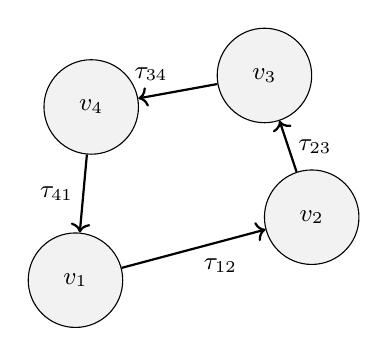
\begin{tikzpicture}[
    neuron/.style={circle, draw=black, fill=gray!10, minimum size=1.2cm, font=\small},
    arrow/.style={->, thick},
    delaylabel/.style={font=\scriptsize, inner sep=1pt},
    every node/.style={font=\small}
]

% Neuron nodes
\node[neuron] (A) at (0, 0) {$v_1$};
\node[neuron] (B) at (3, 0.8) {$v_2$};
\node[neuron] (C) at (2.4, 2.6) {$v_3$};
\node[neuron] (D) at (0.2, 2.2) {$v_4$};

% Edges with temporal consistency
\draw[arrow] (A) -- (B) node[midway, below right] {\( \tau_{12} \)};
\draw[arrow] (B) -- (C) node[midway, right] {\( \tau_{23} \)};
\draw[arrow] (C) -- (D) node[midway, above left] {\( \tau_{34} \)};
\draw[arrow] (D) -- (A) node[midway, left] {\( \tau_{41} \)};

% Caption
%\node at (1.5, -1.1) {\textbf{Figure:} A polychronous neural group as a 1-cycle in \( \mathcal{K}_\delta \)};

\end{tikzpicture}
\caption{A 1-cycle formed by four neurons firing in a delay-consistent sequence, closing to form a reproducible polychronous group. Each edge satisfies the temporal constraint \( |t_j - (t_i + \tau_{ij})| < \delta \).}
\label{fig:1-cyle}
\end{figure}

The preceding lemma characterizes a PNG as a nontrivial 1-cycle in the spatiotemporal complex \( \mathcal{K}_\delta \), emphasizing the topological structure of temporally consistent spike sequences. However, this cyclic characterization appears stricter than the original definition by Izhikevich~\cite{izhikevich2006polychronization}, which permits acyclic but reproducible sequences of delay-locked activations. To reconcile this apparent discrepancy, we observe that the cyclic form can emerge naturally in the presence of recurrent connectivity \cite{schuster1997bidirectional}. 
Recurrent neural architectures, both artificial and biological, inherently support the formation of cycles due to feedback connectivity. Unlike feedforward networks, recurrence enables information to loop through the network, creating directed paths that revisit previously active neurons. 

When such loops are temporally structured, e.g., supported by fixed axonal delays and integration thresholds, they form polychronous sequences that satisfy the cycle condition \( \partial_1(\gamma) = 0 \) in the spatiotemporal complex. These sequences, when non-contractible, define nontrivial homology classes \( [\gamma] \in H_1 \), providing a formal topological foundation for memory encoding via recurrent dynamics \cite{yu2019review}.
When such recurrent paths exist and timing constraints are relaxed slightly, an open PNG sequence can be extended to a closed loop within a larger tolerance window. This leads to the following lemma, which establishes the equivalence between the classical PNG concept \cite{izhikevich2006polychronization} and its topological formulation as a closable, delay-consistent 1-cycle in a filtered complex.

\begin{lemma}[Cycle Completion of Polychronous Sequences]
Let \( \gamma = (v_1 \to v_2 \to \cdots \to v_n) \) be a PNG in the original Izhikevich sense~\cite{izhikevich2006polychronization}, i.e., a temporally precise spike sequence supported by axonal delays and synaptic integration. Under mild assumptions of recurrent connectivity and bounded delay variability, there exists a tolerance \( \delta' > \delta \) and an extension of \( \gamma \) to a closed, temporally consistent 1-cycle \( \gamma' = \gamma \cup \{v_n \to v_1\} \) in the filtered spatiotemporal complex \( \mathcal{K}_{\delta'} \), such that:
$[\gamma'] \in H_1(\mathcal{K}_{\delta'}) \setminus \{0\}$.
In this extended view, PNGs correspond to potentially closable spike trajectories that define topologically persistent memory traces once embedded in recurrent architectures. Thus, the delta-homology formulation subsumes the original PNG definition by interpreting cyclic closure as an idealized limit of stable polychronous activation under recurrent reinforcement.
\label{lemma:equiv}
\end{lemma}

\noindent\textbf{Memory as Nontrivial 1-Cycles}. The result of Lemma~\ref{lemma:equiv} bridges the classical view of PNGs as open, temporally precise spike chains with the homological framework of delta-encoded memory. By demonstrating that polychronous sequences can be extended into closed cycles within a tolerance-adjusted complex \( \mathcal{K}_{\delta'} \), we reinterpret the Izhikevich PNG as a homological seed of latent memory structure. This reinterpretation opens the door to a richer understanding of memory formation: rather than viewing PNGs as isolated motifs, we can now consider their potential for composition and integration. In biologically realistic settings, recurrent connectivity and temporally overlapping activations frequently lead to the chaining of multiple PNGs \cite{st2015implications}. These interactions can generate composite 1-cycles in a larger spatiotemporal complex, encoding not just individual episodes but structured, hierarchical memory traces. This motivates a broader topological perspective on memory, in which persistent loops emerge from the fusion of simpler sequences, as formalized in the following result.

Lemmas \ref{lemma:PNG} and \ref{lemma:equiv} establish that PNGs can be formally identified with nontrivial 1-cycles in the spatiotemporal complex \( \mathcal{K}_\delta \), providing a topological characterization of reproducible, delay-locked neural activity. However, in biological systems, memory is not limited to isolated spike chains; it often involves the dynamic integration of multiple temporally overlapping patterns \cite{buzsaki2010neural}. When two or more PNGs are activated in close succession, their respective chains may become compositionally linked, forming a larger and coherent trajectory through the latent space \cite{fiete2010spike}. Such composition becomes possible when the axonal delay between the endpoint of one chain and the beginning of another lies within an expanded timing window \( \delta' > \delta \). This observation leads to the following lemma, which characterizes the conditions under which two PNGs can fuse into a higher-order cycle, supporting hierarchical memory growth and binding across time \cite{hasson2015hierarchical}.


\begin{lemma}[Temporal Composition of PNGs]
Let \( \gamma_1 = (v_1 \to v_2 \to \cdots \to v_k) \) and \( \gamma_2 = (u_1 \to u_2 \to \cdots \to u_m) \) be two polychronous chains in the spatiotemporal complex \( \mathcal{K}_\delta \), valid under timing tolerance \( \delta \).
Suppose there exist neurons \( v_k \in \gamma_1 \) and \( u_1 \in \gamma_2 \) such that the delayed spike from \( v_k \) reaches \( u_1 \) within an extended timing window \( \delta' > \delta \):
$|t_{u_1} - (t_{v_k} + \tau_{v_k u_1})| < \delta'$.
Then \( \gamma_3 = \gamma_1 \cup \gamma_2 \cup \{v_k \to u_1\} \) is a valid larger PNG in \( \mathcal{K}_{\delta'} \). If further connections close the loop (e.g., \( u_m \to v_1 \)), \( \gamma_3 \) forms a composite 1-cycle in \( H_1(\mathcal{K}_{\delta'}) \).
This mechanism allows for hierarchical memory growth via timing-resolved composition of sub-PNGs.
\label{lemma:TC_PNG}
\end{lemma}

\begin{figure}[h]
\centering
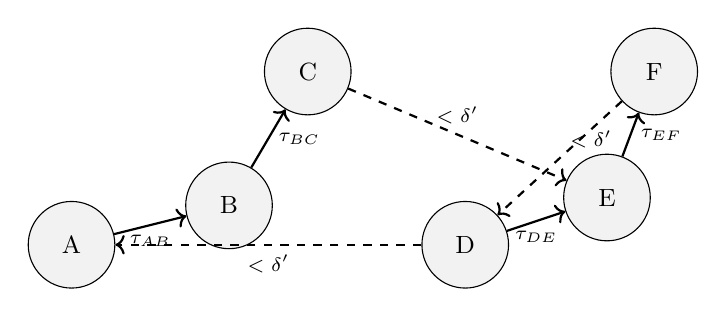
\begin{tikzpicture}[
    neuron/.style={circle, draw=black, fill=gray!10, minimum size=1.1cm, font=\small},
    arrow/.style={->, thick},
    connector/.style={->, thick, dashed},
    label/.style={font=\scriptsize},
    merge/.style={circle, draw=red, fill=red!20, minimum size=0.4cm}
]

% Neurons
\node[neuron] (A) at (0, 0) {A};
\node[neuron] (B) at (2, 0.5) {B};
\node[neuron] (C) at (3, 2.2) {C};

\node[neuron] (D) at (5, 0) {D};
\node[neuron] (E) at (6.8, 0.6) {E};
\node[neuron] (F) at (7.4, 2.2) {F};

% PNG 1
\draw[arrow] (A) -- (B) node[midway, below] {\scriptsize $\tau_{AB}$};
\draw[arrow] (B) -- (C) node[midway, right] {\scriptsize $\tau_{BC}$};

% PNG 2
\draw[arrow] (D) -- (E) node[midway, below] {\scriptsize $\tau_{DE}$};
\draw[arrow] (E) -- (F) node[midway, right] {\scriptsize $\tau_{EF}$};

% Merged edges (appear at higher delta)
\draw[connector] (C) -- (E) node[midway, above] {\scriptsize $< \delta'$};
\draw[connector] (F) -- (D) node[midway, above right] {\scriptsize $< \delta'$};
\draw[connector] (D) -- (A) node[midway, below] {\scriptsize $< \delta'$};

% Loop indication
%\path[draw=none] (A) -- node[below=2.2cm] {\textbf{Composite PNG emerges at higher tolerance \( \delta' \)}} (F);

\end{tikzpicture}
\caption{Two small PNGs (A–B–C and D–E–F) become delay-compatible at a higher timing threshold \( \delta' \), forming a larger polychronous cycle (A–B–C–E–F–D–A). Dashed arrows represent new valid transitions made possible by increased tolerance.}
\label{fig:two_PNG}
\end{figure}

Fig. \ref{fig:two_PNG} depicts an example of a composite PNG emerging at a higher tolerance $\delta'>\delta$. Lemma~\ref{lemma:TC_PNG} highlights how polychronous sequences can merge into larger, hierarchically nested spike motifs, provided their constituent delays remain within an expanded timing window. This motivates the need for a structured framework to accommodate such variable timing constraints and to support topological inference over spike dynamics at multiple resolutions \cite{lin2024topology}. 
To this end, we introduce the \emph{filtered spatiotemporal complex} \( \mathcal{K}_\Delta^\delta \), which generalizes \( \mathcal{K}_\delta \) by incorporating both a spike timing tolerance \( \delta \) and a maximum delay bound \( \Delta \). This complex enables persistent homology to be computed across scales, capturing topologically invariant features, such as reproducible cycles of polychronous activity, that persist under timing jitter and composition \cite{lutgehetmann2020computing}. The formal definition follows.

\begin{definition}[Filtered Spatiotemporal Complex \( \mathcal{K}_\Delta^\delta \)]
Let \( \mathcal{G} = (V, E, \tau) \) be a directed graph of neurons with axonal delay map \( \tau: E \to \mathbb{R}_{>0} \), and let \( \{t_i\}_{i \in V} \) denote observed spike times. Fix a timing tolerance \( \delta > 0 \) and a maximum delay threshold \( \Delta > 0 \).
Define the \emph{filtered spatiotemporal complex} \( \mathcal{K}_\Delta^\delta \) as the directed simplicial complex (or directed flag complex) where:
\begin{itemize}
    \item Vertices are spike events \( i \in V \),
    \item A directed edge \( (i \to j) \in E \) is included if it satisfies both:
   $ |t_j - (t_i + \tau_{ij})| < \delta \quad \text{and} \quad \tau_{ij} \leq \Delta$,
    \item Higher-dimensional simplices are included whenever all lower-order faces (subsequences) satisfy the above consistency and delay constraints.
\end{itemize}
The complex \( \mathcal{K}_\Delta^\delta \) thus encodes all temporally valid activation chains of length bounded by \( \Delta \), filtered by tolerance \( \delta \). It forms the geometric domain for persistent topological inference over spike timing patterns.
\label{def:filtered_spatiotemporal_complex}
\end{definition}


A key observation is that PNGs correspond to 1-cycles in \( \mathcal{K}_\Delta^\delta \) (Lemma~\ref{lemma:PNG}). However, not all 1-cycles encode meaningful memory: some are trivial boundaries of 2-chains (e.g., spike triplets with no temporal specificity). The first homology group \( H_1(\mathcal{K}_\Delta^\delta) \) classifies equivalence classes of such cycles, retaining only those that are nontrivial and topologically robust. Memory in biological systems is not merely a passive record of events, but a structured, compositional, and often path-dependent phenomenon \cite{giusti2015clique}. In temporally precise neural circuits with recurrent connectivity and fixed axonal delays, polychronous activity emerges as reproducible, delay-locked spike sequences that trace dynamic trajectories through latent cognitive space. Capturing the invariant structure of these trajectories requires a framework that is both combinatorial and topological \cite{edelsbrunner2010computational}. To this end, we model the spatiotemporal complex \( \mathcal{K}_\Delta^\delta \) as a chain complex and analyze its homology.

\subsection{Chain Complex and Homology of Spiking Trajectories}

The temporal composition of PNGs, as characterized in Lemma~\ref{lemma:TC_PNG}, highlights the dynamic and hierarchical nature of memory formation in neural circuits: polychronous sequences are not isolated motifs, but modular elements capable of merging into longer, time-locked structures \cite{hasson2015hierarchical}. To systematically capture the global organization of such spike-based dynamics, we interpret the spatiotemporal complex \( \mathcal{K}_\Delta^\delta \), constructed from temporally consistent spike transitions, as the underlying combinatorial scaffold for a chain complex \( (C_*, \partial_*) \). This allows us to formally identify invariant memory structures, such as nontrivial PNG loops, using the language of homology \cite{hatcher2005algebraic}. Through this perspective, each temporally consistent edge becomes a 1-chain, and each closed spike sequence corresponds to a 1-cycle whose topological significance is determined by its (non-)triviality in homology.

\begin{figure}[h]
\centering
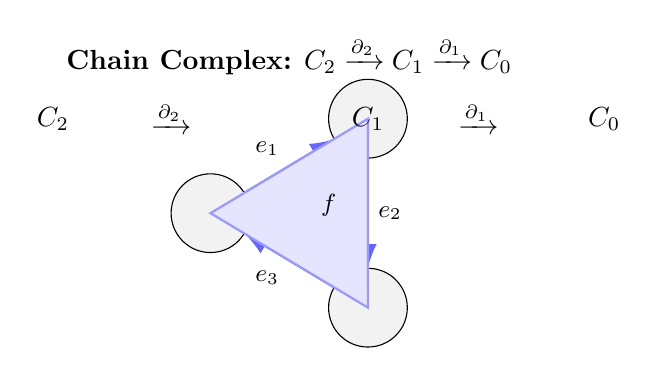
\begin{tikzpicture}[
    node distance=2cm,
    vertex/.style={circle, draw=black, fill=gray!10, minimum size=1cm},
    edge/.style={draw=blue!60, thick, -{Latex[length=3mm]}},
    triangle/.style={fill=blue!10, draw=blue!40, thick},
    label/.style={font=\small}
]

% Vertices
\node[vertex, label=above:$v_1$] (v1) at (0,0) {};
\node[vertex, label=above:$v_2$] (v2) at (2,1.2) {};
\node[vertex, label=below:$v_3$] (v3) at (2,-1.2) {};

% Edges
\draw[edge] (v1) -- (v2) node[midway, above left, label] {$e_1$};
\draw[edge] (v2) -- (v3) node[midway, right, label] {$e_2$};
\draw[edge] (v3) -- (v1) node[midway, below left, label] {$e_3$};

% Triangle
\fill[triangle] (v1.center) -- (v2.center) -- (v3.center) -- cycle;
\node at (1.5,0.1) {\small $f$};

% Chain complex arrows
\node at (-2,1.2) {$C_2$};
\node at (-0.5,1.2) {$\xrightarrow{\partial_2}$};
\node at (3.4,1.2) {$\xrightarrow{\partial_1}$};
\node at (5,1.2) {$C_0$};

% Chain group labels
\node at (1,2) {\textbf{Chain Complex:} $C_2 \xrightarrow{\partial_2} C_1 \xrightarrow{\partial_1} C_0$};
%\node at (1,2.1) {$C_2 \xrightarrow{\partial_2} C_1 \xrightarrow{\partial_1} C_0$};

% Node for C1
\node at (2,1.2) {$C_1$};

\end{tikzpicture}
\caption{A portion of the spatiotemporal complex \( \mathcal{K}_\Delta^\delta \) with vertices \( v_i \in C_0 \), temporally consistent edges \( e_j \in C_1 \), and higher-order timing motif (triangle) \( f \in C_2 \). The boundary operators \( \partial_2 \) and \( \partial_1 \) map 2-chains to their edges and 1-chains to their vertices, respectively. Nontrivial 1-cycles like \( e_1 + e_2 + e_3 \) generate \( H_1(\mathcal{K}_\Delta^\delta) \).}
\label{fig:chain_complex}
\end{figure}

\noindent\textbf{Homology Generators as Structural Memory Units.}
To uncover the topological invariants of neural dynamics, we associate \( \mathcal{K}_\Delta^\delta \) with a \emph{chain complex} \( (C_*, \partial_*) \). This is a sequence of abelian groups (or vector spaces over \( \mathbb{Z}_2 \)) connected by boundary operators:
$\cdots \xrightarrow{\partial_{k+1}} C_k \xrightarrow{\partial_k} C_{k-1} \xrightarrow{\partial_{k-1}} \cdots \xrightarrow{\partial_1} C_0 \to 0$,
such that \( \partial_k \circ \partial_{k+1} = 0 \). As shown in Fig. \ref{fig:chain_complex}, we have:
1) \textbf{\( C_0 \)}: 0-chains, corresponding to spike events (vertices).
2) \textbf{\( C_1 \)}: 1-chains, corresponding to temporally valid spike transitions (edges).
3) \textbf{\( C_2 \)}: 2-chains, representing higher-order timing motifs (e.g., temporal triangles).
The set of \emph{1-cycles}, defined as \( \ker \partial_1 \), consists of closed spike sequences (potential polychronous loops). The set of \emph{1-boundaries}, \( \operatorname{im} \partial_2 \), captures trivial loops that bound a higher-order temporal simplex (i.e., not meaningful PNGs). The quotient
$H_1(\mathcal{K}_\Delta^\delta) := \ker \partial_1 / \operatorname{im} \partial_2$
then gives the first homology group, each class representing a distinct, topologically nontrivial PNG.
The boundary operators \( \partial_k: C_k \rightarrow C_{k-1} \) satisfy \( \partial_k \circ \partial_{k+1} = 0 \), and define cycles and boundaries as follows \cite{bredon2013topology}:
\begin{align}
    Z_k &:= \ker \partial_k \quad \text{(closed chains, or \( k \)-cycles)}, \\
    B_k &:= \operatorname{im} \partial_{k+1} \quad \text{(trivial chains, or \( k \)-boundaries)}.
\end{align}
The \( k \)-th homology group is then given by:
$H_k(\mathcal{K}_\Delta^\delta) := Z_k / B_k = \ker \partial_k / \operatorname{im} \partial_{k+1}$,
which captures the space of topologically distinct \( k \)-dimensional cycles modulo boundaries \cite{spanier2012algebraic}.
The first homology group \( H_1(\mathcal{K}_\Delta^\delta) \) classifies topologically distinct loops of temporally consistent spike activity. Each nontrivial homology class \( [\gamma] \in H_1 \) represents a reproducible, closed trajectory through the spatiotemporal complex. 
These \emph{homology generators} form the atomic building blocks of memory representations in the proposed model. They exhibit three key properties that make them biologically meaningful:

\begin{enumerate}
    \item \textbf{Persistence under Timing Jitter:} 
    Because homology is invariant under small deformations of the underlying complex, the loop \( \gamma \) remains in the same homology class even when spike times vary slightly within the tolerance window \( \delta \). This captures the biological reality that neuronal systems tolerate millisecond-scale variability yet maintain stable memory traces. This robustness aligns with findings in persistent homology, where features with long lifetimes across filtration thresholds are interpreted as noise-resistant structures \cite{edelsbrunner2010computational,ghrist2008barcodes}.

    \item \textbf{Irreducibility:} 
    A homology generator cannot be decomposed into a sum of simpler cycles that are themselves boundaries. This implies that \( \gamma \) encodes a \emph{minimal} nontrivial unit of temporal coordination. In the context of PNGs, this means that the entire loop must be traversed to reinstantiate the memory, partial activation does not suffice. This matches experimental observations where sequence completion, rather than local cue activation, triggers recall \cite{pastalkova2008internally,buzsaki2010neural}.

    \item \textbf{Path-Dependence:} 
    Memory activation depends not just on co-activation of constituent neurons, but on the ordered traversal of a temporal cycle. This property captures the directional, sequence-sensitive nature of episodic memory and behavioral routines. Biological circuits such as CA3 recurrent loops in the hippocampus or reverberatory thalamo-cortical circuits exhibit precisely this kind of loop-based reactivation \cite{mcclelland1995there,buzsaki2006rhythms}. In this framework, the memory trace \( \delta_\gamma \) is only reactivated when the spike trajectory matches the full structure of \( \gamma \), closing the topological loop.
\end{enumerate}

Taken together, these properties establish homology generators as biologically plausible \emph{memory primitives}: sparse, stable, and context-dependent representations that arise from the topology of neural dynamics rather than from specific encoding mechanisms \cite{saggar2018towards}. They function as symbolic attractors in latent space and are ideally suited for implementing inference over structured, temporally extended episodes. This topological perspective invites a deeper formalization of how memory unfolds in time and accounts for the intrinsic temporality embedded in neural sequences. %While homology classes capture the persistence and irreducibility of memory traces, they do not yet account for the intrinsic temporality embedded in neural sequences. %Unlike synchronous assemblies that emphasize co-activation, polychronous neural groups (PNGs) trace directed, time-locked activation paths through latent cognitive spaces \cite{sohn2021network}. To represent this temporal order and compositional structure rigorously, we introduce the abstraction of \emph{cell posets}: partially ordered sets where each cell encodes a spike-timed event or transition, and the covering relations reflect causal precedence. 
\begin{example}[Homology Generator from Recurrent Spiking Pattern]
Consider a recurrent neural microcircuit consisting of four neurons \( \{A, B, C, D\} \) with directed, delay-sensitive synaptic connections:
$A \xrightarrow{\tau_{AB}} B \xrightarrow{\tau_{BC}} C \xrightarrow{\tau_{CD}} D \xrightarrow{\tau_{DA}} A$.
Each connection is activated if the spike from the presynaptic neuron arrives within a fixed delay tolerance \( \delta \) of the expected arrival time, forming a closed, delay-consistent loop.
Let \( \mathcal{K}_\delta \) be the directed spatiotemporal complex constructed from spike-timing data under the tolerance \( \delta \). The above sequence defines a 1-chain
$\gamma = (A \rightarrow B) + (B \rightarrow C) + (C \rightarrow D) + (D \rightarrow A) \in C_1(\mathcal{K}_\delta; \mathbb{F})$.
Since this path is closed and temporally valid, it satisfies \( \partial_1(\gamma) = 0 \), so \( \gamma \in \ker \partial_1 \).
Suppose there are no 2-simplices in \( \mathcal{K}_\delta \) formed from subsets of \( \{A, B, C, D\} \) that could make \( \gamma \) a boundary (e.g., no simultaneously coactive triplets that fill in a triangle). Then \( \gamma \notin \operatorname{im} \partial_2 \), and hence
$[\gamma] \in H_1(\mathcal{K}_\delta)$
is a nontrivial homology class (i.e., a homology generator).
This generator \( [\gamma] \) represents a persistent, reproducible memory trace: the system encodes not just the sequence of activations, but the loop structure that enables recursive traversal and reinforcement. As such, \( [\gamma] \) serves as a structural memory unit, capable of being reactivated when partial contextual cues match any subpath of the cycle.
This topological encoding is robust to noise and partial degradation because it is nonlocal and non-interpolable: it cannot be reduced to a sum of shorter chains or inferred from co-firing statistics alone. Instead, it reflects a fundamental loop in the network’s dynamics.
\end{example}

\begin{tcolorbox}[colback=blue!5, colframe=blue!60!black, title=From Spatiotemporal Complexes to Chain Complexes: a Topological View of Polychronous Neural Groups]
A spatiotemporal complex encodes spike sequences that respect the axonal delay structure of the network. Mapping this to a chain complex allows extraction of homology groups that classify persistent, reproducible spike-timing patterns. Each element of \( H_1(\mathcal{K}_\Delta^\delta) \) corresponds to a temporally closed, topologically irreducible PNG. In this formalism, a polychronous group  corresponds to a 1-cycle in the spatiotemporal complex that is closed under delay-respecting transitions, survives small perturbations in spike timing, and not reducible to a boundary. These polychronous 1-cycles serve as generators of \( H_1 \), and can be interpreted as the topological primitives of neural memory. Overlapping cycles induce intersecting homology classes, enabling compositional reuse of neurons across different functional sequences.
\end{tcolorbox}


\section{Combinatorial Compression of Topological Dynamics}
\label{sec:combi}

Unlike synchronous assemblies, PNGs represent time-locked activation trajectories through latent sensorimotor spaces \cite{sohn2021network}. Their combinatorial and causal structure makes them amenable to abstraction as \emph{cell posets}, which provide a compact topological framework for representing activation order, reproducibility, and overlapping memory traces. This combinatorial scaffold captures both the reproducibility of PNGs and the way in which distinct memory traces can overlap and recombine, laying the groundwork for structured inference over temporally extended episodes \cite{ayzenberg2025sheaf}.

%\subsection{From Spike Sequences to Partially Ordered Sets}

\noindent\textbf{Cell Posets as Temporal Skeletons of Overlapping PNGs.}
A PNG corresponds to a closed, reproducible sequence through a directed \emph{spatiotemporal complex} \( \mathcal{K}_\Delta^\delta \), where each edge encodes a synaptic connection with temporally consistent delay. When multiple PNGs overlap, i.e., they share neurons or time-locked spike events, their structure cannot be represented as a single linear sequence \cite{bredon1997sheaf}. Instead, it gives rise to a natural \emph{partial order}, reflecting both causal precedence and resource reuse.
To formalize this, we define a \emph{cell poset} \( \mathcal{P} \) as follows:

\begin{definition}[Cell Poset]
Let \( \mathcal{K}_\Delta^\delta \) be the spatiotemporal complex encoding delay-locked spike chains, and let \( \Sigma \) be the set of active cells (0-cells for spikes, 1-cells for edges, etc.). Define the cell poset \( \mathcal{P} = (\Sigma, \leq) \) as a partially ordered set where
1) Each element \( \sigma \in \Sigma \) is a cell in \( \mathcal{K}_\Delta^\delta \), representing a spike event, a synaptic transition, or a higher-order motif;
2) The relation \( \sigma \leq \tau \) holds if cell \( \sigma \) causally contributes to \( \tau \), e.g., a spike precedes and enables a subsequent edge, or a chain segment leads into a PNG;
3) A \emph{chain} in \( \mathcal{P} \) is a totally ordered subset \( \sigma_1 < \sigma_2 < \cdots < \sigma_k \), corresponding to a feasible time-respecting spike sequence.
\end{definition}

\begin{figure}[h]
\centering
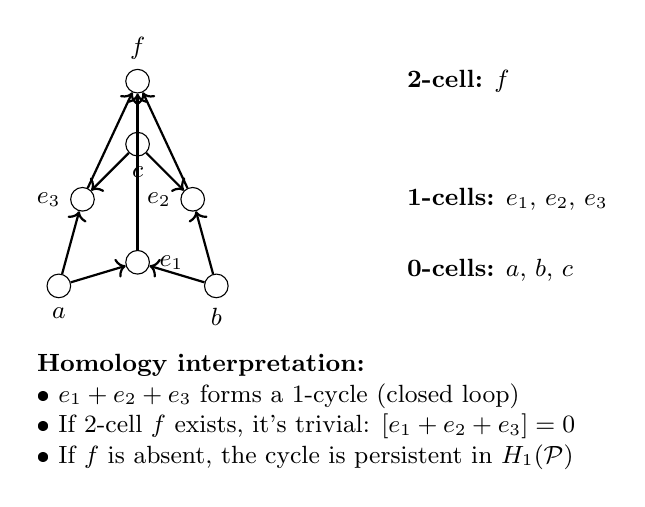
\begin{tikzpicture}[
    node/.style={circle, draw=black, fill=gray!10, minimum size=1cm},
    edge/.style={->, thick},
    hasse/.style={circle, draw=black, fill=white, inner sep=1pt, minimum size=0.3cm},
    font=\small
]

% 0-cells (spikes)
\node[hasse,label=below:$a$] (a) at (0,0) {};
\node[hasse,label=below:$b$] (b) at (2,0) {};
\node[hasse,label=below:$c$] (c) at (1,1.8) {};

% 1-cells (transitions)
\node[hasse,label=right:$e_1$] (e1) at (1,0.3) {};
\node[hasse,label=left:$e_2$] (e2) at (1.7,1.1) {};
\node[hasse,label=left:$e_3$] (e3) at (0.3,1.1) {};

% 2-cell (filled triangle)
\node[hasse,label=above:$f$] (f) at (1,2.6) {};

% Poset edges (cover relations)
\draw[edge] (a) -- (e1);  % a < e1
\draw[edge] (b) -- (e1);  % b < e1

\draw[edge] (b) -- (e2);  % b < e2
\draw[edge] (c) -- (e2);  % c < e2

\draw[edge] (c) -- (e3);  % c < e3
\draw[edge] (a) -- (e3);  % a < e3

\draw[edge] (e1) -- (f);  % e1 < f
\draw[edge] (e2) -- (f);  % e2 < f
\draw[edge] (e3) -- (f);  % e3 < f

% Annotations
\node[draw=none, anchor=west] at (4.3,2.6) {\textbf{2-cell:} $f$};
\node[draw=none, anchor=west] at (4.3,1.1) {\textbf{1-cells:} $e_1$, $e_2$, $e_3$};
\node[draw=none, anchor=west] at (4.3,0.2) {\textbf{0-cells:} $a$, $b$, $c$};

\node[draw=none, align=left, anchor=west] at (-0.4,-1.6) {
    \textbf{Homology interpretation:} \\
    • $e_1 + e_2 + e_3$ forms a 1-cycle (closed loop) \\
    • If 2-cell $f$ exists, it's trivial: $[e_1 + e_2 + e_3] = 0$ \\
    • If $f$ is absent, the cycle is persistent in $H_1(\mathcal{P})$
};

\end{tikzpicture}
\caption{Persistent memory as homology of cell posets. Elements of the cell poset (0-cells, 1-cells, 2-cells) form a chain complex. The 1-cells \( e_1, e_2, e_3 \) form a closed loop over the 0-cells \( a, b, c \). If a 2-cell \( f \) fills this loop, the 1-cycle is trivial in homology. Otherwise, the cycle persists in \( H_1(\mathcal{P}) \), representing a nontrivial memory trace.}
\label{fig:explicit_cycle_cell_poset}
\end{figure}

This poset encodes both 1) \textbf{temporal causality:} The ordering \( \sigma \leq \tau \) respects axonal delays and spike timing constraints;
and 2) \textbf{neural resource reuse:} A single spike event (0-cell) may participate in multiple PNGs, giving rise to branching in the poset structure \cite{wachs2006poset}.
Importantly, the cell poset provides a \emph{discrete combinatorial skeleton} over which topological inference can be performed. Homology classes of chains in \( \mathcal{P} \) correspond to persistent, reproducible memory units that transcend individual activation episodes. Building on this interpretation, the cell poset \( \mathcal{P} \) provides more than a discrete encoding of PNG activation; it admits a natural algebraic structure through which memory dynamics can be analyzed topologically \cite{miller2020homological}. By assigning each cell (spike event, transition, composite activation) a corresponding dimension, we obtain a graded structure over \( \mathbb{F}=\mathbb{Z}_2 \) in which temporal precedence and resource reuse translate into boundary relations. These covering relations induce a boundary operator \( \partial_k \), making \( \mathcal{P} \) a candidate for a chain complex \cite{ayzenberg2025sheaf}. Homology then reveals which spike trajectories are persistent and irreducible, those that are not boundaries of higher-dimensional composites. The following lemma formalizes this correspondence.


\begin{lemma}[Chain Complex from Cell Poset]
Let \( \mathcal{P} \) be a finite cell poset formed from overlapping PNGs, where each element corresponds to a cell of dimension \( k \in \{0,1,2,\dots\} \) representing a temporally ordered activation unit (e.g., spike, edge, triangle). Then \( \mathcal{P} \) defines a graded chain complex \( (C_*, \partial_*) \) over a field \( \mathbb{F}=\mathbb{Z}_2  \), with:
1) \( C_k \) the \( \mathbb{F} \)-vector space generated by the set of \( k \)-cells in \( \mathcal{P} \);
2) \( \partial_k: C_k \to C_{k-1} \) the boundary map induced by the covering relations \( \sigma^{(k-1)} < \tau^{(k)} \) in the poset;
3) Satisfying \( \partial_k \circ \partial_{k+1} = 0 \) for all \( k \).
The homology groups \( H_k(\mathcal{P}) := \ker \partial_k / \operatorname{im} \partial_{k+1} \) then encode persistent topological features of the cell poset structure, such as reproducible 1-cycles corresponding to PNG memory traces.
\label{lemma:chain_complex_cell_poset}
\end{lemma}


\begin{figure}[h]
\centering
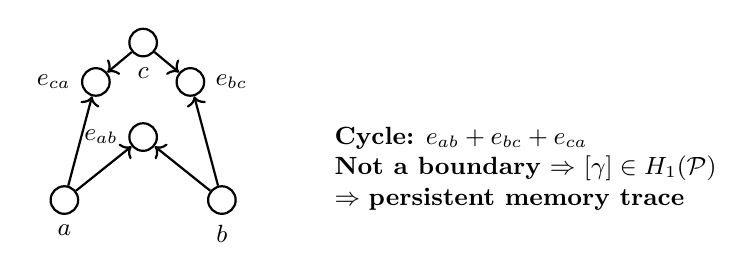
\begin{tikzpicture}[
    node/.style={circle, draw=black, fill=gray!10, minimum size=1cm},
    edge/.style={->, thick},
    hasse/.style={circle, draw=black, fill=white, inner sep=1pt, minimum size=0.35cm},
    every path/.style={draw, thick},
    font=\small
]

% 0-cells
\node[hasse,label=below:$a$] (a) at (0,0) {};
\node[hasse,label=below:$b$] (b) at (2,0) {};
\node[hasse,label=below:$c$] (c) at (1,2) {};

% 1-cells (edges)
\node[hasse,label=left:$e_{ab}$] (e1) at (1,0.8) {};
\node[hasse,label=right:$e_{bc}$] (e2) at (1.6,1.5) {};
\node[hasse,label=left:$e_{ca}$] (e3) at (0.4,1.5) {};

% Poset arrows
\draw[edge] (a) -- (e1);
\draw[edge] (b) -- (e1);

\draw[edge] (b) -- (e2);
\draw[edge] (c) -- (e2);

\draw[edge] (c) -- (e3);
\draw[edge] (a) -- (e3);

% No 2-cell here — cycle is nontrivial
\node[draw=none, align=left, anchor=west] at (3.3,0.4) {
    \textbf{Cycle:} $e_{ab} + e_{bc} + e_{ca}$ \\
    \textbf{Not a boundary} $\Rightarrow$ $[\gamma] \in H_1(\mathcal{P})$ \\
    $\Rightarrow$ \textbf{persistent memory trace}
};

\end{tikzpicture}
\caption{A nontrivial 1-cycle in the cell poset: the edges $e_{ab}$, $e_{bc}$, and $e_{ca}$ form a closed loop with no corresponding 2-cell to bound them. This irreducible, path-dependent activation pattern defines a persistent homology class in \( H_1(\mathcal{P}) \), interpreted as a stable memory trace.}
\label{fig:nontrivial_cycle_cell_poset}
\end{figure}

Building on Lemma~\ref{lemma:chain_complex_cell_poset}, we now interpret the resulting homological structure in functional terms. The graded chain complex \( (C_*, \partial_*) \) derived from the cell poset \( \mathcal{P} \) supports a principled representation of memory architecture: 0-cells represent spike events, 1-cells correspond to temporally consistent transitions, and higher-dimensional cells encode recurrent motifs and compositions \cite{izhikevich2006polychronization}. Within this framework, 1-cycles in \( \ker \partial_1 \) capture closed, reproducible spike patterns, precisely the structure of PNGs. However, only those cycles that are not boundaries of higher-dimensional activations, i.e., elements of \( H_1(\mathcal{P}) = \ker \partial_1 / \operatorname{im} \partial_2 \), qualify as persistent memory traces. These nontrivial homology classes reflect path-dependent, irreducible, and temporally structured units of neural computation \cite{giusti2015clique}. The cell poset's topology thus embeds not only temporal causality but also structural memory constraints, enabling compositional reuse of subpatterns across overlapping PNGs \cite{sizemore2019importance}. This persistent structure evolves under changes in the temporal resolution \( \delta \), forming a filtration that can be analyzed through persistent homology \cite{edelsbrunner2008persistent} to identify topologically stable memory features.


\begin{figure}[h]
\centering
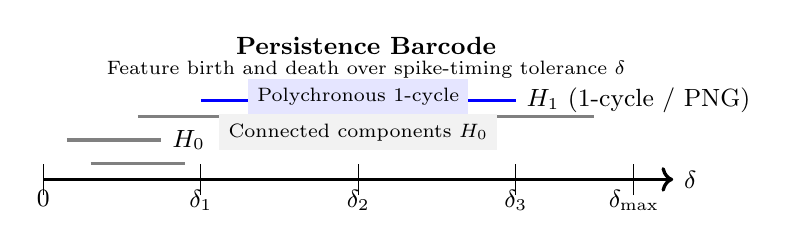
\begin{tikzpicture}[
    axis/.style={very thick, ->},
    bar/.style={very thick},
    tick/.style={thin},
    font=\small
]

% Axes
\draw[axis] (0,0) -- (8,0) node[anchor=west] {\( \delta \)};
\draw (0,-0.2) -- (0,0.2) node[below=6pt] {\( 0 \)};
\draw (2,-0.2) -- (2,0.2) node[below=6pt] {\( \delta_1 \)};
\draw (4,-0.2) -- (4,0.2) node[below=6pt] {\( \delta_2 \)};
\draw (6,-0.2) -- (6,0.2) node[below=6pt] {\( \delta_3 \)};
\draw (7.5,-0.2) -- (7.5,0.2) node[below=6pt] {\( \delta_{\text{max}} \)};

% Bars
\draw[bar, blue] (2,1) -- (6,1) node[right, black] {\( H_1 \) (1-cycle / PNG)};
\draw[bar, gray] (0.3,0.5) -- (1.5,0.5) node[right, black] {\( H_0 \)};
\draw[bar, gray] (0.6,0.2) -- (1.8,0.2);
\draw[bar, gray] (1.2,0.8) -- (7.0,0.8);

% Legend
\node at (4.1, 1.7) {\textbf{Persistence Barcode}};
\node at (4.1, 1.4) {\scriptsize Feature birth and death over spike-timing tolerance \( \delta \)};
\node[draw=none, fill=blue!10, text=black] at (4., 1.05) {\scriptsize Polychronous 1-cycle};
\node[draw=none, fill=gray!10, text=black] at (4., 0.6) {\scriptsize Connected components \( H_0 \)};

\end{tikzpicture}
\caption{Persistence barcode of a spatiotemporal complex under increasing timing tolerance \( \delta \). The blue bar indicates a 1-cycle (corresponding to a polychronous group) that is born at \( \delta_1 \), persists through \( \delta_2 \), and dies at \( \delta_3 \). Bars in gray represent connected components in \( H_0 \).}
\label{fig:persistent_barcode}
\end{figure}

\noindent\textbf{Persistent Memory as Homology of Cell Posets.}
The cell poset \( \mathcal{P} \) supports a natural homological structure:
\begin{itemize}
    \item Chains in the poset form the basis of a chain complex \( (C_*, \partial_*) \),
    \item PNGs correspond to 1-cycles \( c \in \ker \partial_1 \),
    \item Persistent memory traces are those cycles not contractible to a boundary: \( H_1(\mathcal{P}) = \ker \partial_1 / \operatorname{im} \partial_2 \).
\end{itemize}
Overlapping PNGs induce intersecting cycles in the poset, supporting compositionality and reuse of neurons across functional memory patterns. As temporal tolerance \( \delta \) varies, this structure can be filtered to extract topologically robust features via persistent homology \cite{edelsbrunner2008persistent}. 

\begin{figure*}[h]
\centering
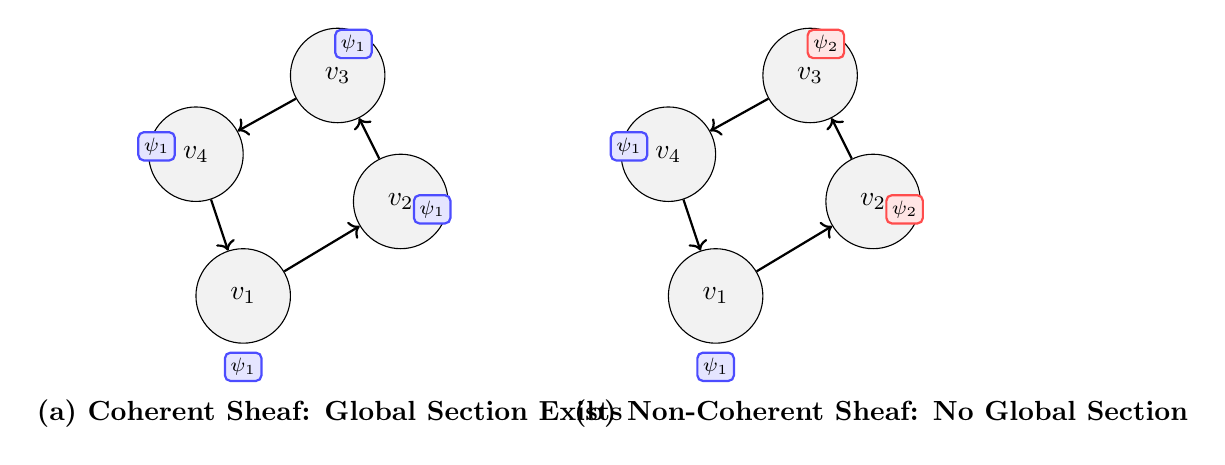
\begin{tikzpicture}[
    cell/.style={circle, draw=black, fill=gray!10, minimum size=1.2cm},
    edge/.style={->, thick},
    label/.style={font=\small},
    sheaf/.style={draw=blue!70, thick, fill=blue!10, font=\scriptsize, inner sep=2pt, rounded corners=2pt},
    sheaf_conflict/.style={draw=red!70, thick, fill=red!10, font=\scriptsize, inner sep=2pt, rounded corners=2pt}
]

% Left: Coherent case
\node[cell] (A1) at (0,0) {$v_1$};
\node[cell] (B1) at (2,1.2) {$v_2$};
\node[cell] (C1) at (1.2,2.8) {$v_3$};
\node[cell] (D1) at (-0.6,1.8) {$v_4$};

\draw[edge] (A1) -- (B1);
\draw[edge] (B1) -- (C1);
\draw[edge] (C1) -- (D1);
\draw[edge] (D1) -- (A1);

% Sheaf values (coherent)
\node[sheaf] at (0,-0.9) {\( \psi_1 \)};
\node[sheaf] at (2.4,1.1) {\( \psi_1 \)};
\node[sheaf] at (1.4,3.2) {\( \psi_1 \)};
\node[sheaf] at (-1.1,1.9) {\( \psi_1 \)};

\node at (1.1, -1.5) {\textbf{(a) Coherent Sheaf: Global Section Exists}};

% Right: Non-coherent case
\node[cell] (A2) at (6,0) {$v_1$};
\node[cell] (B2) at (8,1.2) {$v_2$};
\node[cell] (C2) at (7.2,2.8) {$v_3$};
\node[cell] (D2) at (5.4,1.8) {$v_4$};

\draw[edge] (A2) -- (B2);
\draw[edge] (B2) -- (C2);
\draw[edge] (C2) -- (D2);
\draw[edge] (D2) -- (A2);

% Sheaf values (conflict)
\node[sheaf] at (6,-0.9) {\( \psi_1 \)};
\node[sheaf_conflict] at (8.4,1.1) {\( \psi_2 \)};
\node[sheaf_conflict] at (7.4,3.2) {\( \psi_2 \)};
\node[sheaf] at (4.9,1.9) {\( \psi_1 \)};

\node at (8.1, -1.5) {\textbf{(b) Non-Coherent Sheaf: No Global Section}};

\end{tikzpicture}
\caption{Coherence via global section. (a) In the coherent case, local context assignments agree across overlaps and can be glued into a global section, enabling successful recall. (b) In the non-coherent case, conflicting local sections prevent global unification, obstructing memory inference.}
\label{fig:coherent_sheaf_cycle}
\end{figure*}


An enlightening distinction in the persistent memory lies in whether a closed spike sequence bounds a higher-order cell. As illustrated in Figure~\ref{fig:explicit_cycle_cell_poset}, the 1-cells \( e_1, e_2, e_3 \) form a closed loop over 0-cells \( a, b, c \), but this loop is bounded by a 2-cell \( f \). In this case, the cycle is a boundary: it belongs to \( \operatorname{im} \partial_2 \), and thus represents a \emph{trivial} element in the first homology group \( H_1(\mathcal{P}) \). Despite its reproducibility, such a cycle is homologically reducible and does not define a persistent memory trace.
By contrast, Figure~\ref{fig:nontrivial_cycle_cell_poset} shows a similar loop formed by edges \( e_{ab}, e_{bc}, e_{ca} \) with no 2-cell to fill it. This structure defines a \emph{nontrivial homology class} in \( H_1(\mathcal{P}) \), corresponding to a sparse, irreducible, and path-dependent memory unit under the delta-homology analogy. It cannot be decomposed into simpler components and persists under timing noise, making it a candidate for long-term storage in the latent inference process \cite{sukhbaatar2019augmenting}.
Though both figures show closed, potentially reproducible polychronous patterns, only the unfilled cycle supports a persistent memory trace. This reflects a key insight of CCUP \cite{li2025CCUP}: \textbf{nontriviality in homology encodes the low-entropy content variable \( \Phi \)}, while trivial cycles may reflect transient contextual scaffolding \( \Psi \).

\begin{theorem}[Homological Characterization of Persistent Memory Traces]
Let \( \mathcal{P} \) be the cell poset formed from overlapping PNGs, and let \( (C_*, \partial_*) \) be the associated chain complex over a field \( \mathbb{F} \). A 1-chain \( \gamma \in C_1(\mathcal{P}) \) represents a persistent memory trace if and only if:
$\gamma \in \ker \partial_1 \quad \text{and} \quad \gamma \notin \operatorname{im} \partial_2$,
i.e., \( [\gamma] \in H_1(\mathcal{P}) \) is a nontrivial homology class.
Such memory traces, corresponding to closed, reproducible polychronous spike sequences are not only irreducible and sparse (they cannot be constructed from smaller homological units)
but also path-dependent and stable under timing jitter, serving as attractors in latent inference.
\label{thm:homological_persistence}
\end{theorem}

\noindent
Theorem~\ref{thm:homological_persistence} provides a rigorous homological criterion for identifying memory traces as nontrivial 1-cycles in the chain complex of the cell poset \( \mathcal{P} \). However, empirical recordings may yield reproducible patterns of spike activity, such as reactivated PNGs, that are not necessarily homologically significant \cite{reimann2017cliques}. Some reproducible 1-cycles may, in fact, bound higher-order simplices and therefore lie in the image of \( \partial_2 \), rendering them topologically trivial.
To distinguish genuinely persistent memory traces from mere recurrence, we introduce a homological filtering principle \cite{ghrist2008barcodes}. This corollary formalizes how the first homology group \( H_1(\mathcal{P}) \) acts as a topological sieve: it selects only those reproducible spike sequences that are irreducible, non-bounding cycles and thereby structurally encoded in the memory substrate.
To quantify the robustness of memory traces under varying spike-timing tolerances, we analyze the persistence of 1-cycles in the cell complex \( \mathcal{P} \). As the timing threshold \( \delta \) increases, new connections emerge, cycles may form or collapse, and the homology structure evolves accordingly. Figure~\ref{fig:persistent_barcode} illustrates this evolution as a persistence barcode: bars in \( H_0 \) represent connected components, while long-lived features in \( H_1 \), such as polychronous 1-cycles, indicate topologically stable memory traces.



\begin{corollary}[Topological Filter for Empirical PNGs]
Let \( \gamma \in C_1(\mathcal{P}) \) be a \emph{reproducible} 1-cycle derived from empirical spike data, such as a reliably reactivated PNG. Then:
1) If \( \gamma \in \operatorname{im} \partial_2 \), then \( [\gamma] = 0 \in H_1(\mathcal{P}) \) and the memory trace is homologically trivial, despite being reproducible;
2) If \( \gamma \notin \operatorname{im} \partial_2 \), then \( [\gamma] \neq 0 \in H_1(\mathcal{P}) \) and the memory trace is topologically persistent.
The homology group \( H_1(\mathcal{P}) \) functions as a filter that separates merely recurrent activity from structurally encoded memory.
\label{cor:homological_filter}
\end{corollary}

The corollary above highlights how homological nontriviality distinguishes structurally encoded memory from transient recurrence. To further formalize the algebraic organization of such traces across the cell poset \( \mathcal{P} \), we introduce a sheaf-theoretic framework that encodes local delta-like memory activations and their global compatibility \cite{ayzenberg2025sheaf}. Specifically, we define a sheaf \( \mathcal{F} \) whose stalks are generated by delta responses \( \delta_\sigma \) at each cell \( \sigma \in \mathcal{P} \). These local sections can be glued into global memory patterns only when their overlaps respect the homological constraints of \( \mathcal{P} \) \cite{sizemore2019importance}. Coherence of the sheaf then characterizes whether local delta traces assemble into persistent, nontrivial memory cycles, leading to the following sheaf-based definition:


\begin{definition}[Sheaf of Delta Memory Traces]
Let \( \mathcal{P} \) be the cell poset of a spatiotemporal complex. Define a presheaf \( \mathcal{F} \) that assigns to each cell \( \sigma \in \mathcal{P} \) a vector space \( \mathcal{F}(\sigma) \) generated by delta-like functions \( \delta_\sigma \). A section over an open set \( U \subseteq \mathcal{P} \) is a collection of such deltas satisfying compatibility over overlaps.
A sheaf \( \mathcal{F} \) is said to be coherent if the delta-traces glue to form nontrivial homology cycles in \( H_1(\mathcal{P}) \), representing persistent memory traces.
\end{definition}

The above definition captures how delta-like spike events can be localized to cells of the poset and assembled into consistent patterns via sheaf-theoretic gluing. Note that not all collections of delta traces yield meaningful memory structures: only those that extend to global sections respecting both temporal causality and cell adjacency induce persistent activity cycles. This motivates a homological interpretation of \emph{coherent} sheaves \cite{grauert2012coherent}: those that glue local delta sections into nontrivial global memory traces. The following theorem formalizes this connection between sheaf coherence and persistent homology:

\begin{theorem}[Coherent Sheaves Encode Persistent Memory Traces]
Let \( \mathcal{P} \) be a finite cell poset formed from overlapping PNGs, and let \( \mathcal{F} \) be a sheaf over \( \mathcal{P} \) such that:
1) For each \( k \)-cell \( \sigma \in \mathcal{P} \), \( \mathcal{F}(\sigma) \) is a finite-dimensional \( \mathbb{F} \)-vector space generated by delta-like activations \( \delta_\sigma \);
2) The restriction maps \( \rho_{\tau\sigma} : \mathcal{F}(\tau) \to \mathcal{F}(\sigma) \) encode boundary relations \( \sigma < \tau \);
3) The sheaf \( \mathcal{F} \) is coherent, i.e., locally finitely generated with finitely generated relations among local sections.
Then the set of global sections \( \Gamma(\mathcal{P}, \mathcal{F}) \) that satisfy the sheaf gluing condition correspond bijectively to 1-cycles \( \gamma \in \ker \partial_1 \subseteq C_1(\mathcal{P}) \). Moreover, if a global section does not lie in the image of the boundary map \( \operatorname{im} \partial_2 \), then it defines a nontrivial homology class \( [\gamma] \in H_1(\mathcal{P}) \), representing a persistent memory trace.
$\boxed{
\text{Coherent sheaf } \mathcal{F} \ \Longrightarrow \ \text{Persistent cycle } [\gamma] \in H_1(\mathcal{P})
}$.
\label{thm:coherent_sheaf_memory}
\end{theorem}

Theorem~\ref{thm:coherent_sheaf_memory} formalizes how coherent sheaves encode persistent memory via nontrivial homology classes. To illustrate this intuitively, we contrast two sheaf configurations over the same cycle of cells. In the coherent case, each local section assigns a delta-like activation (e.g., \( \psi_1 \)) consistently across adjacent cells, allowing the formation of a global section that traverses the entire 1-cycle. In the non-coherent case, conflicting local assignments (e.g., \( \psi_1 \) vs. \( \psi_2 \)) disrupt the sheaf gluing condition, preventing the construction of a global memory trace. This distinction is depicted in Figure~\ref{fig:coherent_sheaf_cycle}, where coherence guarantees persistent inference across the cycle, while incoherence blocks integration of local patterns into a global memory \cite{abramsky2011sheaf}.
The essence of Theorem~\ref{thm:coherent_sheaf_memory} lies in distinguishing the structural role of the cell poset \( \mathcal{P} \) from the informational role of the sheaf \( \mathcal{F} \). While the poset provides the pure combinatorial skeleton, the sheaf enriches this structure by assigning to each cell a space of possible local activations and prescribing how these activations must agree across adjacent cells. A global section exists if and only if these local data assignments satisfy the sheaf's gluing condition: all restriction maps commute along the poset's covering relations. This condition ensures that memory activation is not merely locally plausible but globally coherent. 
In the context of PNGs, a coherent sheaf configuration around a 1-cycle enables a persistent memory trace to emerge, whereas incoherent assignments disrupt global consistency and block recall.
In summary, coherence serves as a structural gatekeeper, converting local activation into global memory via topological alignment \cite{schmid2025applied}.


Together, Theorems \ref{thm:homological_persistence} and~\ref{thm:coherent_sheaf_memory} underscore a critical distinction between local reproducibility and global persistence. While a polychronous sequence may appear reliably across trials, only those sequences whose local sections align coherently, yielding a global, glued configuration, contribute to the structural memory encoded in \( H_1(\mathcal{P}) \). This coherence ensures that the memory trace is not merely an artifact of local correlation but reflects a topologically robust structure that persists across perturbations. The key criterion is homological nontriviality: cycles that do not bound any higher-order cell cannot be collapsed or explained away by simpler components. This leads to the following central insight:


\begin{tcolorbox}[colback=blue!5, colframe=blue!60!black, title=Key Insight: Nontriviality Implies Memory]
Not all reproducible spike sequences represent persistent memory. 
A cycle in the cell poset \( \mathcal{P} \) qualifies as a \emph{persistent memory trace} if and only if it is a \textbf{nontrivial 1-cycle}, i.e., it lies in \( \ker \partial_1 \) but not in \( \operatorname{im} \partial_2 \). 
A coherent sheaf guarantees that a spike pattern can be reconstructed globally, but only when this cycle is homologically nontrivial does it encode a persistent memory trace in the sense of delta-homology. So coherence is necessary for activation, but nontriviality is necessary for persistence. 
In summary, \textbf{nontriviality in homology distinguishes minimal latent memory structures from redundant or interpolated activity}.
\end{tcolorbox}

\begin{figure*}[h]
\centering
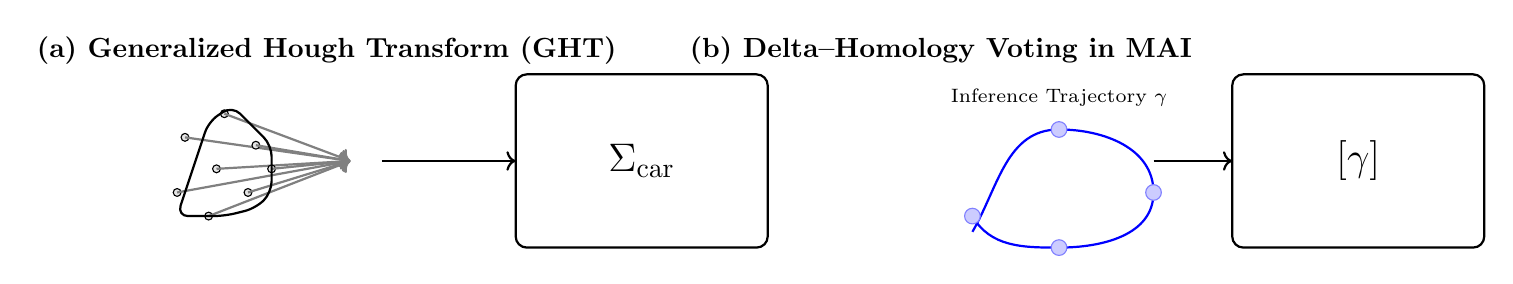
\begin{tikzpicture}[
    edgept/.style={circle, draw=black, fill=gray!20, inner sep=1pt},
    latentpt/.style={circle, draw=blue!50, fill=blue!20, inner sep=2pt},
    accumulator/.style={rounded corners, draw=black, thick, minimum width=3.2cm, minimum height=2.2cm},
    arrow/.style={->, thick},
    caroutline/.style={draw=black, thick, rounded corners},
    vote/.style={->, thick, draw=gray},
    loop/.style={thick, draw=blue},
    label/.style={font=\small}
]

% ===== GHT LEFT =====
\node at (0,3.4) {\textbf{(a) Generalized Hough Transform (GHT)}};

% Edge points (features)
\foreach \x/\y in {-1.8/2.3, -1.3/2.6, -0.9/2.2, -1.0/1.6, -1.5/1.3, -1.9/1.6, -1.4/1.9, -0.7/1.9} {
    \node[edgept] at (\x,\y) {};
    \draw[vote] (\x,\y) -- (0.3,2); % Voting toward template center
}

% Car shape outline
\draw[caroutline] (-1.9,1.3) -- (-1.5,2.5) -- (-1.2,2.7) -- (-0.9,2.4) -- (-0.7,2.2) -- (-0.7,1.6)
 -- (-0.9,1.4) -- (-1.3,1.3) -- cycle;

% Arrow to accumulator
\draw[arrow] (0.7,2) -- (2.4,2);

% Template accumulator
\node[accumulator, label=below:{\small Template Center Accumulator}] at (4,2) {};
\node at (4,2) {\Large $\Sigma_{\text{car}}$};

% ===== DELTA-HOMOLOGY RIGHT =====
\node at (7.8,3.4) {\textbf{(b) Delta–Homology Voting in MAI}};

% Latent cycle (inference loop)
\draw[loop] (8.2,1.1) to[out=60,in=180] (9.3,2.4)
            to[out=0,in=90] (10.5,1.6)
            to[out=270,in=0] (9.3,0.9)
            to[out=180,in=300] (8.2,1.3);

% Loop label
\node at (9.3,2.8) {\scriptsize Inference Trajectory \( \gamma \)};

% Latent points
\foreach \x/\y in {8.2/1.3, 9.3/2.4, 10.5/1.6, 9.3/0.9} {
    \node[latentpt] at (\x,\y) {};
}

% Arrow to accumulator
\draw[arrow] (10.5,2) -- (11.5,2);

% Homology accumulator
\node[accumulator, label=below:{\small Homology Classifier}] at (13.1,2) {};
\node at (13.1,2) {\Large $[\gamma]$};

\end{tikzpicture}
\caption{Comparison of (a) Generalized Hough Transform (GHT) for generic shape detection and (b) Delta–Homology Voting in memory-amortized inference (MAI). In GHT, edge features vote toward a known geometric template (e.g., a car) via a reference point accumulator. In delta–homology, each inference step emits a delta-like activation along a latent cycle \( \gamma \), which triggers a persistent memory only when the full topological loop is reconstructed.}
\label{fig:delta_ght_car}
\end{figure*}

\section{Delta-Homology as a Memory Substrate}
\label{sec:delta}

To formalize the relationship between inference trajectory and structural memory in the latent space, we introduce the \emph{delta-homology analogy}, which connects the emergence of sparse memory traces with generators of the first homology group \( H_1 \) of the sensorimotor manifold \cite{sohn2021network}. This analogy establishes the topological conditions under which a Dirac delta-like trace \cite{richards1995theory} signifies the encoding of an irreducible memory cycle.

\begin{definition}[Delta-Homology Analogy]
Let \( \mathcal{Z} \subset \mathbb{R}^d \) be a latent manifold representing structured cognitive states, and let \( H_1(\mathcal{Z}) \) denote its first homology group over a field \( \mathbb{F} \) (e.g., \( \mathbb{F} = \mathbb{Z}_2 \) or \( \mathbb{R} \)). A closed loop \( \gamma: S^1 \rightarrow \mathcal{Z} \) is called a \emph{homology generator} if its equivalence class \( [\gamma] \in H_1(\mathcal{Z}) \) is nontrivial, that is, \( \gamma \) is not the boundary of any 2-chain in \( \mathcal{Z} \).
We define the \emph{delta-homology analogy} as follows: a Dirac delta-like memory trace \( \delta_\gamma \) corresponds to a pure generator \( [\gamma] \in H_1(\mathcal{Z}) \) if
(i) \( \delta_\gamma \) is sharply localized along \( \gamma \); 
(ii) memory activation occurs if and only if the inference trajectory completes the full cycle \( \gamma \);
In this analogy, \( \delta_\gamma \) is interpreted as a sparse, irreducible, and non-interpolable memory unit encoding the topological signature of the loop \( \gamma \). Such traces serve as minimal, path-dependent attractors in memory-amortized inference and cannot be synthesized from local features alone.
\end{definition}

The delta-homology analogy provides a principled topological framework for interpreting memory traces as nontrivial cycles on a latent manifold. To make this concept concrete, we now consider a canonical example from systems neuroscience: the periodic activity patterns of grid cells in the medial entorhinal cortex \cite{moser2015place}. These cells tile physical space with a hexagonal lattice, and their periodicity induces a compact topological structure on the latent representation space \cite{stemmler2015connecting}. Under suitable boundary conditions, this space is naturally modeled as a flat torus \( \mathbb{T}^2 \), on which spatial trajectories induce looped latent cycles. As we show below, such loops instantiate homology generators, and their completion activates sparse delta-like traces corresponding to structured memory units. %This illustrates how grid cells realize the delta-homology mechanism in a biologically grounded setting:


\begin{example}[Grid Cells and Delta-Homology on the Torus]
Grid cells in the medial entorhinal cortex exhibit periodic spatial firing patterns that tile the environment in a hexagonal lattice. Let the physical space be modeled as a compact domain \( \Omega \subset \mathbb{R}^2 \), and let the activity of a grid cell be represented by a sharply localized function \( \delta_{x_i} \) centered at preferred locations \( \{x_i\} \subset \Omega \).
Under periodic boundary conditions, the phase space of grid cell activity can be topologically modeled as a flat 2-torus \( \mathbb{T}^2 = S^1 \times S^1 \), where each point on the torus corresponds to a spatial phase (offset) of the grid code \cite{stemmler2015connecting}. A movement trajectory in physical space induces a trajectory \( \gamma: S^1 \to \mathbb{T}^2 \) on this latent manifold.
In the delta-homology analogy, each full traversal around the torus along a non-contractible loop corresponds to a homology generator \( [\gamma] \in H_1(\mathbb{T}^2) \), and the associated memory trace \( \delta_\gamma \) is activated only if the spatial path completes the full cycle. The superposition
$\delta_\gamma = \sum_{i \in \gamma} \delta_{x_i}$
encodes a sparse, irreducible memory unit that reflects the topological structure of the grid lattice. This trace cannot be reconstructed from any acyclic subpath or partial activation, it requires coherent traversal of the entire loop, reflecting path-dependent integration \cite{mcnaughton2006path}.
%Thus, grid cells naturally instantiate the delta-homology memory mechanism: their periodicity creates a toroidal latent space, while their activation encodes topologically nontrivial cycles, allowing for structure-aware spatial memory and navigation.
\end{example}


The delta-homology analogy provides a geometric and algebraic bridge between sparse, loop-like memory encodings and their underlying topological generators. By interpreting Dirac delta-like activations as signatures of nontrivial homology classes, we gain a language for describing irreducible, path-dependent memory units that resist interpolation \cite{rosiak2022sheaf}. This framework naturally extends to the analysis of PNGs, whose reproducible spatiotemporal structure forms discrete cycles in the filtered complex \( \mathcal{K}_\delta \). The following lemma formalizes this correspondence, showing how each closed PNG trajectory admits a delta-like memory representation that functions as a topological generator in \( H_1(\mathcal{K}_\delta) \).


\begin{lemma}[Delta-Homology Interpretation of PNGs]
Let \( \gamma \subset \mathcal{K}_\delta \) be a directed 1-cycle corresponding to a PNG, as characterized in Lemma~\ref{lemma:PNG}. Then the delta-homology analogy assigns to \( \gamma \) a localized memory trace \( \delta_\gamma \), such that:
1) \( \delta_\gamma \) is sharply supported on the neurons and transitions participating in \( \gamma \),
2) \( \delta_\gamma \) is activated \emph{if and only if} an inference trajectory completes the full cycle \( \gamma \),
3) \( \delta_\gamma \) defines a generator of the first homology group \( H_1(\mathcal{K}_\delta) \), and cannot be synthesized from any acyclic or interpolated subpath of \( \gamma \),
4) In the CCUP framework, \( \delta_\gamma \) represents a low-entropy, path-dependent content unit \( \Phi \), whose accessibility is gated by coherent high-entropy context \( \Psi \).
\label{lemma:DHI_PNG}
\end{lemma}

Under the delta-homology analogy, PNGs are interpreted as topological memory primitives whose activation dynamics are sparse, temporally compositional, and irreducible to static representations.
The delta-homology interpretation of PNGs provides a localized description of how reproducible neural trajectories encode memory as topological invariants \cite{izhikevich2006polychronization}. More importantly, this viewpoint scales from individual cycles \( \gamma \subset \mathcal{K}_\delta \) to the entire homological structure of the cell poset \( \mathcal{P} \), where overlapping PNGs collectively generate a chain complex of delta-supported activations. Each edge in a 1-cycle contributes a delta-like basis element \( \delta_e \), and memory traces emerge as sparse superpositions of such activations \cite{dicarlo2012does}. The following theorem formalizes this lifting, establishing precise algebraic conditions under which these delta-composed chains define persistent memory units in \( H_1(\mathcal{P}) \).


\begin{theorem}[Delta-Homology Representation of Memory Traces]
Let \( \mathcal{P} \) be a finite cell poset formed from overlapping PNGs, and let \( (C_*, \partial_*) \) be its associated chain complex over the field \( \mathbb{F} = \mathbb{Z}_2 \). Then:
1) Each directed 1-cell (edge) \( e \in C_1(\mathcal{P}) \) can be represented by a delta-like activation functional \( \delta_e \), sharply localized along a spike transition;
2) A memory trace \( \gamma \in C_1(\mathcal{P}) \) corresponds to a sparse superposition:
$\gamma = \sum_{e \in E} \delta_e$;
where the sum is taken over a closed, temporally consistent chain of edges forming a 1-cycle.
3) This trace defines a persistent memory unit if and only if
$\gamma \in \ker \partial_1 \quad \text{and} \quad \gamma \notin \operatorname{im} \partial_2$,
i.e., the homology class \( [\gamma] \in H_1(\mathcal{P}) \) is nontrivial.
\label{thm:delta_homology_representation}
\end{theorem}

Under this representation, delta-like functionals serve as algebraic memory primitives, sparse, localized, irreducible, and structurally coupled to topological features of the underlying spatiotemporal dynamics.
Theorem~\ref{thm:delta_homology_representation} formalizes how memory traces arise as sparse, delta-like 1-cycles in the chain complex of a cell poset, grounding persistent memory in the algebraic structure of homology. To extend this idea from discrete neural chains to inference over continuous latent spaces, we reinterpret these delta-supported traces as topological templates for structured recall. Specifically, we draw an analogy to the Generalized Hough Transform (GHT) \cite{ballard1981generalizing}, where latent trajectories induced by the inference cycle serve as deformable and robust templates. The following proposition reframes \( \delta_\gamma \) as a topological generalization of GHT: instead of accumulating spatial votes for geometric alignment, it accumulates contextual evidence over latent trajectories, activating only when the global cycle is coherently completed. %This construction reveals how memory-amortized inference (MAI) retrieves structure not through local interpolation but through globally persistent, path-dependent homology classes.

\begin{example}[Place Cells and Delta-Homology in Spatial Trajectories]
Place cells in the hippocampus activate when an animal occupies specific locations in its environment. Let the explored environment be modeled as a 2D domain \( \Omega \subset \mathbb{R}^2 \), and define a filtered spatiotemporal complex \( \mathcal{K}_\Delta^\delta \) over the animal’s trajectory, where vertices correspond to spike events, and edges are added when temporal differences match known axonal delays within tolerance \( \delta \). Each place cell activation \( \delta_{x_i} \) is sharply localized at spatial position \( x_i \in \Omega \) and time \( t_i \).
When the animal revisits locations to form a closed spatial path (e.g., running a loop), the sequence of coactivated place cells traces a nontrivial 1-cycle \( \gamma_{\text{place}} \in H_1(\mathcal{K}_\Delta^\delta) \), representing a persistent spatial memory \cite{tversky2005functional}. The delta-homology trace associated with this trajectory is
$\delta_{\gamma_{\text{place}}} = \sum_{i \in \gamma_{\text{place}}} \delta_{x_i}$,
which encodes a sparse, topologically stable memory trace. This trace cannot be reconstructed from any non-looping subpath and is reactivated only upon complete traversal of the spatial loop, reflecting path-dependent encoding consistent with hippocampal replay and remapping phenomena \cite{o1978hippocampus, wilson1994reactivation}.
\end{example}


\begin{corollary}[Delta–Homology as a Topological Generalization of the GHT]
Let \( \mathcal{Z} \subset \mathbb{R}^d \) be a compact latent manifold representing structured memory states. Let \( \gamma: S^1 \to \mathcal{Z} \) be a latent trajectory induced by inference cycles such that:
1) \( \gamma \) forms a closed loop with nontrivial homology class \( [\gamma] \in H_1(\mathcal{Z}) \);
2) Each inference step emits a latent state \( \Phi^{(i)} \in \mathcal{Z} \), mapped from context \( \Psi^{(i)} \) via inverted inference;
3) A memory trace \( \delta_\gamma \) is sharply supported on \( \gamma \), and is activated iff the inference trajectory completes the loop \( \gamma \) up to tolerance \( \delta \ll 1 \).
Then the following holds:
1) The memory trace \( \delta_\gamma \) acts as a topological generalization of the Generalized Hough Transform: it accumulates contextual votes \( \Psi^{(i)} \mapsto \Phi^{(i)} \) that align with \( \gamma \), and activates only upon full cycle completion.
2) The activation of \( \delta_\gamma \) is invariant under noise in context \( \Psi \), provided the inference path remains in the homology class \( [\gamma] \), thus ensuring topological robustness.
3) This process implements a \emph{structure-aware retrieval mechanism} within MAI: rather than interpolating from local neighbors, memory is retrieved by identifying persistent cycles that generalize across noisy contexts.
4) Therefore, \( \delta_\gamma \) represents the topological analog of a parametric template in GHT, where persistent homology replaces rigid geometric matching, and inference-driven loops replace spatial voting.
\label{cor:delta_ght}
\end{corollary}

To visually contrast the classical spatial voting of the GHT with the topological inference dynamics of delta–homology, Figure~\ref{fig:delta_ght_car} provides a side-by-side illustration. In panel~(a), GHT detects object templates, such as a car silhouette, by accumulating local edge features, each casting a vote in a shared parametric accumulator space. The final template is retrieved when sufficient geometric consensus is reached. In panel~(b), delta–homology memory operates over a latent manifold \( \mathcal{Z} \), where each inference step produces a latent state \( \Phi^{(i)} \in \mathcal{Z} \) aligned with a target cycle \( \gamma \). The memory trace \( \delta_\gamma \) is activated only when the inference path completes the entire loop up to a small tolerance \( \delta \), ensuring that retrieval is invariant to contextual noise yet precise in topological structure. Thus, delta–homology generalizes the GHT framework from geometric voting to structure-aware retrieval, where memory is indexed not by parametric templates, but by persistent homology classes.


This shift from spatial feature accumulation to latent cycle completion underscores a deeper structural unification: what the GHT achieves via geometric consensus in Euclidean space, delta–homology achieves via topological coherence on latent manifolds. Crucially, this generalization requires more than just matching local features, it demands that those features be stitched together through a globally consistent structure. This role is played by the sheaf \( \mathcal{F} \) over the cell poset \( \mathcal{P} \), where coherence ensures that delta-supported activations align across overlaps to form a persistent 1-cycle. The following proposition formalizes this correspondence, showing that when the sheaf is coherent, the resulting global section \( \delta_\gamma \) defines a nontrivial homology class and supports structure-aware memory retrieval akin to, but topologically deeper than, template matching in GHT.


\begin{proposition}[Coherent Sheaf Enables Delta-Homology Memory Activation]
Let \( \mathcal{P} \) be a cell poset formed from spike-timed activations, and let \( \mathcal{F} \) be a coherent sheaf assigning delta-like local sections \( \delta_\sigma \) to cells \( \sigma \in \mathcal{P} \). Then:
1) The global section \( \delta_\gamma \in \Gamma(\mathcal{P}, \mathcal{F}) \) formed by gluing compatible local delta activations defines a 1-chain \( \gamma \in C_1(\mathcal{P}) \);
2) If \( \gamma \in \ker \partial_1 \) and \( \gamma \notin \operatorname{im} \partial_2 \), then \( [\gamma] \in H_1(\mathcal{P}) \) is a persistent memory trace;
3) The delta-trace \( \delta_\gamma \) functions as a structure-aware template, generalizing the Generalized Hough Transform: it accumulates inference votes \( \Psi^{(i)} \mapsto \Phi^{(i)} \) that match the loop \( \gamma \), and activates only upon coherent completion.
\end{proposition}

The proposition above formalizes how coherent sheaves encode structured memory by gluing local delta-like activations into a globally consistent 1-cycle, triggering persistent retrieval only when contextual input aligns with a stored topological template. To ground this abstract mechanism in biological cognition, we now turn to a concrete neurophysiological instantiation: concept cells \cite{quiroga2005invariant}. These cells provide a vivid example of delta-homology memory in action, where disparate sensory inputs are integrated into a unified, concept-specific memory trace. The example below illustrates how the coherent sheaf construction captures this integration process and how the resulting global section encodes a homologically nontrivial memory representation.


\begin{example}[Concept Cells as Coherent Sheaf Activations]
Concept cells in the human medial temporal lobe respond selectively to high-level semantic entities, such as a specific person, place, or idea, regardless of the sensory modality through which the concept is cued \cite{quiroga2012concept}. Let \( \mathcal{P} \) be the cell poset formed from spike-timed responses to various multimodal cues (e.g., image, name, voice) associated with a concept. Define a coherent sheaf \( \mathcal{F} \) over \( \mathcal{P} \), assigning delta-like local sections \( \delta_\sigma \) to each modality-specific activation cell \( \sigma \in \mathcal{P} \).
When a consistent set of sensory cues (e.g., viewing a photo of Jennifer Aniston, hearing her name, and reading her biography) jointly satisfy the gluing conditions of the sheaf, they assemble into a global section \( \delta_\gamma \in \Gamma(\mathcal{P}, \mathcal{F}) \). This section defines a 1-chain \( \gamma \in C_1(\mathcal{P}) \) that represents the integrated concept. If \( \gamma \in \ker \partial_1 \) and \( \gamma \notin \operatorname{im} \partial_2 \), then the corresponding homology class \( [\gamma] \in H_1(\mathcal{P}) \) encodes a persistent memory trace for the concept.
Under the delta-homology analogy, the concept cell acts as a structure-aware template matcher, akin to a generalized Hough transform: it accumulates votes from distributed input features, and fires only when the inputs form a coherent cycle aligned with the stored template \( \gamma \). %Thus, concept cells naturally implement delta-homology memory via coherent sheaf activation.
\end{example}



\begin{tcolorbox}[colback=blue!5, colframe=blue!60!black, title=Key Bridge: Sheaf Coherence $\rightarrow$ Delta-Homology $\rightarrow$ Topological Template Matching]
A \textbf{coherent sheaf} of delta-like spike activations enables the construction of a global memory trace \( \delta_\gamma \) that 1) glues together local activations into a full 1-cycle;
2) represents a nontrivial homology class \( [\gamma] \in H_1(\mathcal{P}) \);
 3) acts as a topological template, activated only when inference completes the matching cycle;
4) generalizes the GHT to latent manifolds with structured memory.
\end{tcolorbox}


\section{Memory-Amortized Inference over Delta-Homology Structures}
\label{sec:MAI}

The CCUP posits that cognition arises from the dynamic alignment between two distinct types of latent variables: a low-entropy \emph{content variable} \( \Phi \), and a high-entropy \emph{context variable} \( \Psi \) \cite{li2025CCUP}. These two components play complementary roles in structuring inference: while \( \Phi \) encodes the stable, internally simulated content of experience, \( \Psi \) governs the uncertainty, generalization, and flexibility necessary for adaptive interpretation and behavior. To operationalize this alignment, Memory-Amortized Inference (MAI) leverages the sparsity and recurrence of delta-like activations supported on nontrivial homology classes of latent structure, enabling efficient recall and integration of past experience through topologically grounded memory cycles.

\begin{figure*}[h]
\centering
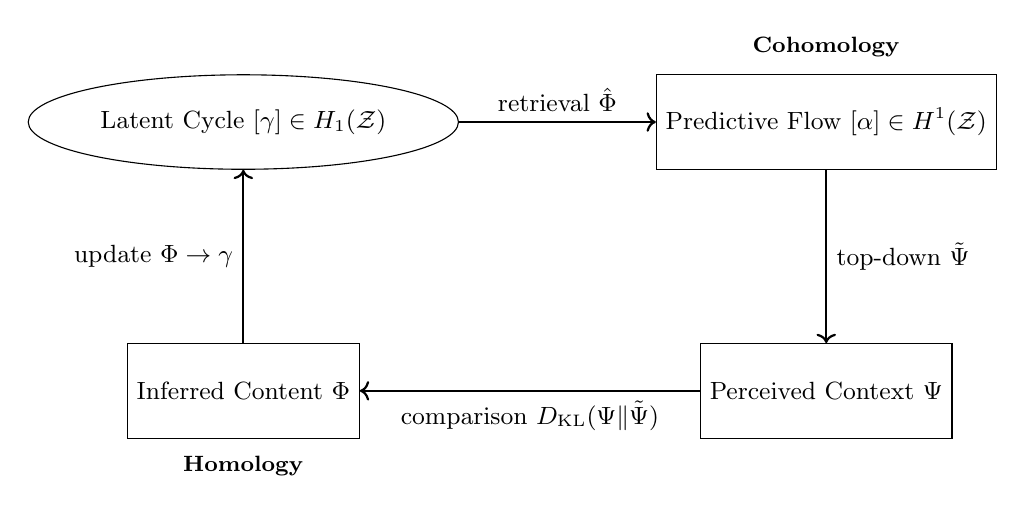
\begin{tikzpicture}[
    node distance=2.2cm and 2.5cm,
    every node/.style={font=\small},
    state/.style={draw, ellipse, minimum width=2.8cm, minimum height=1.2cm},
    box/.style={draw, rectangle, minimum width=2.8cm, minimum height=1.2cm},
    arrow/.style={->, thick},
    dashedarrow/.style={->, thick, dashed}
]

% Nodes
\node[state] (memory) {Latent Cycle $[\gamma] \in H_1(\mathcal{Z})$};
\node[box, right=of memory] (prediction) {Predictive Flow $[\alpha] \in H^1(\mathcal{Z})$};
\node[box, below=of prediction] (perception) {Perceived Context $\Psi$};
\node[box, below=of memory] (inference) {Inferred Content $\Phi$};

% Arrows
\draw[arrow] (memory) -- node[above] {retrieval $\hat{\Phi}$} (prediction);
\draw[arrow] (prediction) -- node[right] {top-down $\tilde{\Psi}$} (perception);
\draw[arrow] (perception) -- node[below] {comparison $D_{\mathrm{KL}}(\Psi \| \tilde{\Psi})$} (inference);
\draw[arrow] (inference) -- node[left] {update $\Phi \to \gamma$} (memory);

% Cycle Label
\node[below =0.1cm and 0.3cm of inference, font=\footnotesize] {\textbf{Homology}};
\node[above =0.1cm and -0.4cm of prediction, font=\footnotesize] {\textbf{Cohomology}};

\end{tikzpicture}
\caption{Predictive inference as a homology–cohomology loop. Memory cycles guide perception; prediction errors modulate memory through topological alignment.}
\end{figure*}

\noindent\textbf{Content as Persistent Topological Structure.}
The content variable \( \Phi \) is characterized by low entropy and high structural stability. It represents the internalized, persistent features of experience, what is remembered, reconstructed, or simulated across time. Mathematically, \( \Phi \) is represented by topological invariants derived from the activity space, such as 1) Homology groups \( H_k(\mathcal{K}) \) over a simplicial or spatiotemporal complex \( \mathcal{K} \); 2) Persistent homology barcodes (refer to Fig. \ref{fig:persistent_barcode}), identifying stable topological features across filtration scales; 3) PNGs represented as homology generators in the neural activation space.
These features define reproducible latent cycles and compositional structures that serve as the basis for inference. Once inferred, \( \Phi \) is resistant to noise and perturbation, and serves as a scaffold for latent prediction, motor planning, and memory consolidation \cite{petri2014homological}.

\noindent\textbf{Context as Filtration, Cohomology, or Sheaf.}
In contrast, the context variable \( \Psi \) is high-entropy, dynamic, and distributed. It determines \emph{when}, \emph{where}, and \emph{under what conditions} the content \( \Phi \) should be activated, interpreted, or suppressed. Context is not represented as a fixed structure but rather as a modulating field over latent space, with the following equivalent mathematical representations:
1) \textbf{Filtration function:} a scalar-valued function over a complex (e.g., time, uncertainty, salience), inducing a filtration that modulates the emergence of topological features \cite{bassett2017network}; 2) \textbf{Cohomology class:} a dual object assigning values (e.g., attention, phase, modulation) to cycles in \( \Phi \), reflecting which latent features are activated in a given setting \cite{bredon1997sheaf}; 3) \textbf{Sheaf:} an assignment of local data or uncertainty to each open set or cell in a poset, encoding how contextual information varies across space and time \cite{brown2020sheaf}.
These representations allow context to dynamically gate, weight, or restrict the inference pathways through the latent content space. When consistent, \( \Psi \) supports coherent inference by selecting a globally valid interpretation; when fragmented, it leads to ambiguity, conflict, or hallucination \cite{varela2017embodied}.

\noindent\textbf{Context–Content Duality as Inference Principle.}
The content–context decomposition is not merely a modeling convenience, but a functional necessity for efficient inference. Under CCUP, content \( \Phi \) is retrieved or simulated via persistent structures, low-entropy attractors in latent space and context \( \Psi \) modulates which parts of \( \Phi \) are activated, assigning relevance, accessibility, or plausibility.
It follows that inference unfolds as a cycle between context and content, minimizing their joint uncertainty while preserving structural consistency.
This duality maps naturally onto algebraic topology:
\begin{align*}
    \Phi &\in H_k(\mathcal{K}) \quad &&\text{(homology: structure of content)} \\
    \Psi &\in H^k(\mathcal{K}, \mathcal{F}) \quad &&\text{(cohomology: modulation by context)}
\end{align*}
The sheaf \( \mathcal{F} \) encodes how local interpretations vary, and whether a globally coherent state of inference exists. When \( H^1(\mathcal{F}) = 0 \), the context is coherent and globally consistent; otherwise, the system may be unable to integrate local priors into a unified perception.


The above decomposition sets the stage for understanding memory recall as a consistency problem between latent structure and contextual modulation. When content \( \Phi \) is encoded as a nontrivial homology class \( [\gamma] \in H_1(\mathcal{K}) \), its successful retrieval depends on whether the surrounding context \( \Psi \in H^1(\mathcal{K}, \mathcal{F}) \) supports a coherent interpretation. Specifically, contextual sections must align across overlapping regions to form a global section that consistently activates the underlying memory trace. If such a global section exists, the system can stably recall \( \gamma \); if not, recall fails due to contextual incoherence. This interplay between homology and cohomology \cite{iversen2012cohomology} operationalizes the context–content duality as a structural gating condition for memory access. The following lemma formalizes this principle by identifying coherent recall with the existence of a global section in the contextual sheaf \( \mathcal{F} \).


\begin{lemma}[Coherent Recall Requires a Global Section]
Let \( \mathcal{P} \) be a cell poset formed from temporally ordered spike events (e.g., polychronous sequences), and let \( \mathcal{F} \) be a sheaf assigning contextual values to the elements of \( \mathcal{P} \), with restriction maps preserving inference consistency across overlaps.
Suppose a homology generator \( [\gamma] \in H_1(\mathcal{P}) \) represents a candidate memory trace. Then successful recall of \( \gamma \) occurs if and only if there exists a \emph{global section} \( s \in \Gamma(\mathcal{P}, \mathcal{F}) \) such that
$\forall U \subseteq \mathcal{P}, \quad s|_U = s_U$,
where \( \{s_U\} \) are the locally assigned contextual sections over each patch \( U \) covering \( \gamma \). If no such global section exists, recall fails due to contextual incoherence, and \( \gamma \) remains latent or ambiguous.
In this setting, failure to recall corresponds to the existence of a nontrivial cohomology class:
$H^1(\mathcal{F}) \ne 0$,
which obstructs the gluing of local inferences into a coherent memory representation.
\label{lemma:coherent_recall}
\end{lemma}

Lemma~\ref{lemma:coherent_recall} establishes that successful memory recall requires the existence of a global section over the sheaf \( \mathcal{F} \), ensuring that local inferences along a candidate cycle \( \gamma \in H_1(\mathcal{P}) \) are contextually consistent. Since sheaves are about interaction between local and global properties of geometric objects, this consistency criterion extends beyond isolated cycles: when multiple feature-specific 1-cycles \( \{\gamma_i\} \) coexist within the neural substrate, recall of a composite memory depends on the compatibility of their local sections on shared overlaps. In this way, the sheaf-theoretic gluing condition becomes a principled mechanism for \emph{binding} \cite{treisman1980feature}, the construction of higher-order memory representations by temporally composing multiple latent cycles. The following proposition formalizes this idea, showing that when contextual values align across a union of partially overlapping polychronous groups, a global section emerges that coherently binds their individual contributions into a unified memory trace.


\begin{proposition}[Feature Binding via Temporal Composition and Sheaf Gluing]
Let \( \mathcal{P} \) be a cell poset of spike-time events, and let \( \mathcal{F} \) be a sheaf assigning contextual feature maps to its cells.
Let \( \{\gamma_i\} \) be disjoint 1-cycles (PNGs) encoding distinct features, each admitting local section \( s_i \in \mathcal{F}(\gamma_i) \). Suppose a composite cycle \( \gamma^* = \cup_i \gamma_i \cup \{e_{ij}\} \) forms under extended temporal tolerance \( \delta' \), introducing overlaps among \( \gamma_i \).
Then if \( \{s_i\} \) are consistent on overlaps in \( \gamma^* \), they glue into a global section \( s \in \Gamma(\mathcal{P}, \mathcal{F}) \). This constitutes successful feature binding under CCUP.
\label{prop:binding}
\end{proposition}

Proposition~\ref{prop:binding} formalizes feature binding \cite{treisman1996binding} as a sheaf-theoretic gluing process: multiple polychronous cycles \( \{\gamma_i\} \) can be temporally composed into a composite memory trace \( \gamma^* \), provided their local contextual inferences are coherent on overlaps. This mechanism ensures that complex representations emerge from temporally extended yet structurally consistent dynamics. However, beyond this constructive view lies a deeper duality intrinsic to the perception–action cycle \cite{sohn2021network}. From the CCUP perspective, inference unfolds as a loop governed by both bottom-up latent memory structure (homology) and top-down predictive modulation (cohomology). The interaction between memory traces \( [\gamma] \in H_1 \) and predictive potentials \( [\alpha] \in H^1 \) yields a natural pairing, evaluating how well predictions align with encoded experience. The following theorem formalizes this duality, showing that inference achieves stability and alignment when the cohomological potential vanishes along memory-supporting cycles \cite{keller2018predictive}. This closes the loop: memory shapes predictions, and prediction filters memory access, thereby grounding cognition in a dual topological architecture.

\begin{figure}[h]
\centering
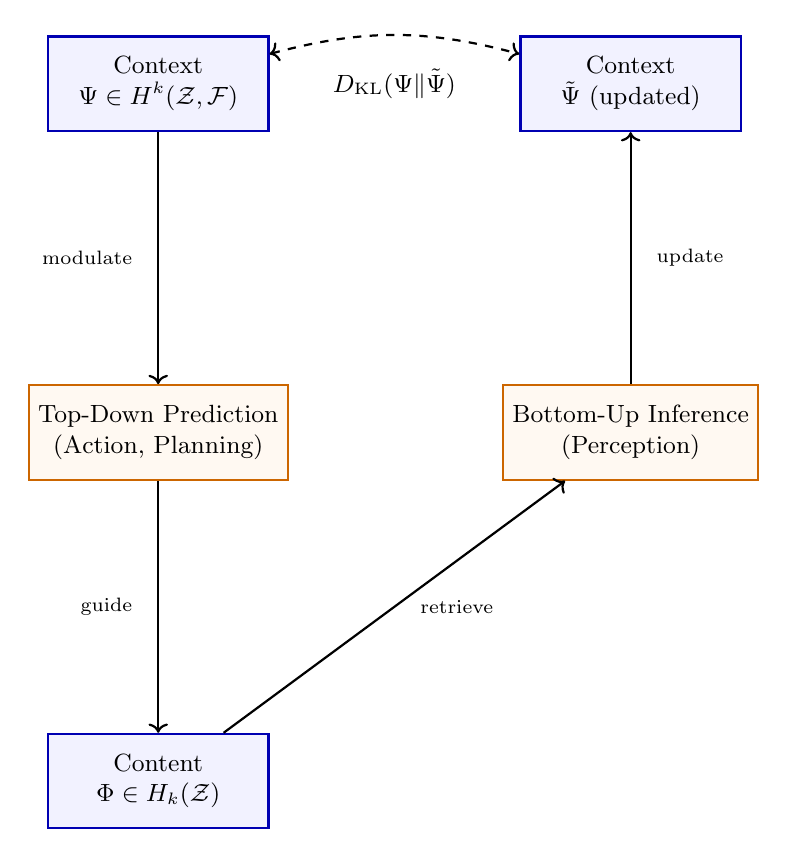
\begin{tikzpicture}[
    node distance=3.2cm and 3.6cm,
    roundnode/.style={draw=blue!70!black, thick, minimum width=2.8cm, minimum height=1.2cm, align=center, fill=blue!5},
    squarenode/.style={draw=orange!80!black, thick, minimum width=3.2cm, minimum height=1.2cm, align=center, fill=orange!5},
    arrow/.style={->, thick},
    dualarrow/.style={<->, thick, dashed},
    font=\small
]

% Nodes
\node[roundnode] (context) {Context \\ \( \Psi \in H^k(\mathcal{Z}, \mathcal{F}) \)};
\node[squarenode, below=of context] (action) {Top-Down Prediction \\ (Action, Planning)};
\node[roundnode, below=of action] (content) {Content \\ \( \Phi \in H_k(\mathcal{Z}) \)};
\node[squarenode, above=of content, xshift=6cm] (perception) {Bottom-Up Inference \\ (Perception)};
\node[roundnode, above=of perception] (context2) {Context \\ \( \tilde{\Psi} \) (updated)};

% Arrows for the cycle
\draw[arrow] (context) -- (action) node[midway, left, xshift=-0.2cm] {\scriptsize modulate};
\draw[arrow] (action) -- (content) node[midway, left, xshift=-0.2cm] {\scriptsize guide};
\draw[arrow] (content) -- (perception) node[midway, right, xshift=0.2cm] {\scriptsize retrieve};
\draw[arrow] (perception) -- (context2) node[midway, right, xshift=0.2cm] {\scriptsize update};
\draw[dualarrow, dashed] (context) to[bend left=15] (context2);

% Optional labels
\node at ($(context)!0.5!(context2)$) {\small \( D_{\mathrm{KL}}(\Psi \| \tilde{\Psi}) \)};
%\node at ($(action)!0.5!(perception)$) [below=1.4cm] {\small Memory-amortized inference loop};

\end{tikzpicture}
\caption{Perception–Action Cycle as a Dual Loop under CCUP–MAI. Context \( \Psi \) modulates inference, content \( \Phi \) encodes memory, and prediction closes the loop through cohomology–homology alignment.}
\label{fig:ccup_dual_loop}
\end{figure}


\begin{theorem}[Homology–Cohomology Dual Loop under CCUP]
Let \( \mathcal{Z} \subset \mathbb{R}^d \) be a compact latent manifold representing structured memory states, and let \( [\gamma] \in H_1(\mathcal{Z}; \mathbb{F}) \) be a nontrivial homology class representing a latent memory cycle and \( [\alpha] \in H^1(\mathcal{Z}; \mathbb{F}) \) be a cohomology class representing a predictive potential (e.g., top-down expectation or reward gradient).
Then under cycle-consistent inference, the perception–action loop satisfies:
$\langle \alpha, \gamma \rangle \approx 0 \quad \Leftrightarrow \quad D_{\mathrm{KL}}(\Psi \| \tilde{\Psi}) \approx 0$,
i.e., prediction and memory are aligned when the cohomological potential evaluated on the homological memory cycle vanishes.
This pairing establishes:
1) Memory stability via \( [\gamma] \in H_1 \): inference loops persist and encode reusable structure;
2) Predictive modulation via \( [\alpha] \in H^1 \): forward models adjust based on mismatch with latent cycles;
3) A closed loop of inference, where top-down predictions guide action and bottom-up experience reinforces memory.
\label{thm:dual_loop}
\end{theorem}

\noindent\textbf{Application to Sensorimotor Learning.}
Theorem~\ref{thm:dual_loop} formalizes how the perception–action loop in sensorimotor learning \cite{fuster2004upper} can be understood as a homology–cohomology duality under the CCUP. In this setting, the latent manifold \( \mathcal{Z} \) encodes structured sensorimotor representations learned over repeated interactions with the environment. A nontrivial homology class \( [\gamma] \in H_1(\mathcal{Z}) \) represents a reusable, temporally extended motor routine, such as a reach or grasp trajectory, whose structure persists across variations \cite{todorov2004optimality}. The corresponding cohomology class \( [\alpha] \in H^1(\mathcal{Z}) \) captures the predictive modulation imposed by task goals, proprioceptive priors, or expected sensory outcomes. The vanishing of the pairing \( \langle \alpha, \gamma \rangle \approx 0 \) indicates that the planned action (top-down prediction) is aligned with the recalled motor memory (bottom-up structure), minimizing the Kullback-Leibler divergence \( D_{\mathrm{KL}}(\Psi \| \tilde{\Psi}) \) between actual and predicted context \cite{cover1999elements}. Hence, learning proceeds by adjusting the predictive cohomology class \( [\alpha] \) to match the homological memory cycle \( [\gamma] \), forming a closed inference loop that supports context-aware motor execution and adaptive refinement. This dual structure provides a topological account of motor habits, error-driven adaptation, and goal-directed behavior in sensorimotor systems \cite{sohn2021network}.



Figure~\ref{fig:ccup_dual_loop} schematizes this inference architecture as a dual loop. The top node \( \Psi \in H^k(\mathcal{Z}, \mathcal{F}) \) represents the current context, formulated cohomologically (e.g., from environmental cues or internal goals). This context modulates top-down prediction (Action), which attempts to activate a content unit \( \Phi \in H_k(\mathcal{Z}) \), typically a motor memory trace retrieved from latent space \cite{sohn2021network}. The system then engages in bottom-up inference (Perception), reconstructing a context \( \tilde{\Psi} \) from the resulting sensory input. The loop closes when the updated context matches the original, formalized as the vanishing of the information discrepancy \( D_{\mathrm{KL}}(\Psi \| \tilde{\Psi}) \approx 0 \), indicating cycle-consistent inference \cite{keller2018predictive}.
Homologically, this alignment means that the cohomological potential vanishes on the memory cycle, \( \langle \alpha, \gamma \rangle \approx 0 \), signifying that top-down plans are structurally compatible with bottom-up recall. This mechanism supports motor learning as a recursive process \cite{todorov2002optimal}: predictive potentials adapt to better align with stable memory cycles, while new experience reinforces the persistence of those cycles. Memory stability is thus governed by \( H_1(\mathcal{Z}) \), predictive plasticity by \( H^1(\mathcal{Z}) \), and their interplay sustains an adaptive sensorimotor loop rooted in delta-homology and sheaf-theoretic coherence. The CCUP framework generalizes this loop as a topological engine of inference, balancing context-driven modulation with content-driven persistence.

\noindent\textbf{Dual of Feature Binding in Motor Control.}
Under the homology–cohomology duality posited by CCUP, feature binding through temporal composition and sheaf gluing in perception corresponds in motor control to trajectory binding via coherent predictive potentials. Whereas feature binding involves assembling delta-like spike activations into nontrivial homology cycles, motor control entails aligning local motor primitives into a globally consistent plan, formalized as a global section in a co-sheaf over the latent space \cite{prinz1997perception}. This predictive potential, represented by a cohomology class \( [\alpha] \in H^1(\mathcal{Z}) \), guides action selection such that its evaluation on a memory cycle \( [\gamma] \in H_1(\mathcal{Z}) \) satisfies \( \langle \alpha, \gamma \rangle \approx 0 \). This vanishing pairing indicates that the action plan is consistent with past experience, enabling cycle-consistent execution and reinforcing the latent memory structure.

This duality completes the sensorimotor loop: just as perception integrates temporally extended spike events into coherent memory cycles through sheaf gluing, motor control integrates predictive potentials into executable trajectories via co-sheaf coherence \cite{friston2010action}. Under the MAI framework, inference proceeds by cycling between these two operations, feature binding (bottom-up) and trajectory binding (top-down), such that memory traces \( [\gamma] \in H_1(\mathcal{Z}) \) serve as latent mediators between context \( \Psi \in H^1(\mathcal{Z}) \) and content \( \Phi \in H_1(\mathcal{Z}) \). Successful inference requires that the gluing condition in the sheaf (perception) and the coherence condition in the co-sheaf (action) are jointly satisfied. When both conditions are met, the system traverses a topologically meaningful cycle in latent space that preserves structure, minimizes uncertainty, and supports behaviorally effective action. Thus, MAI implements a closed-loop architecture in which perception updates context through the completion of homology generators, and action reuses structure through cohomological alignment, forming a cycle-consistent, memory-amortized learning process \cite{heald2021contextual}.


\begin{tcolorbox}[colback=blue!5, colframe=blue!60!black, title=Content–Context Duality under CCUP]
Under the CCUP, the low-entropy content variable \( \Phi \) is captured by persistent homology, stable, topologically invariant structures such as 1-cycles and higher-dimensional features. In contrast, the high-entropy context variable \( \Psi \) is represented dually as a filtration, cohomology class, or sheaf over the same space. A \emph{coherent state} corresponds to a global section of this sheaf: all local contextual assignments are compatible and glue into a unified interpretation; a \emph{non-coherent state} arises when local contexts conflict, preventing global inference. This failure of coherence is quantified by nontrivial sheaf cohomology (e.g., \( H^1(\mathcal{F}) \ne 0 \)), and signals fragmented or ambiguous cognitive states. The perception-action loop implements memory-amortized inference via the duality of persistent topological structure and modulating contextual sheaves.
\end{tcolorbox}

\section{Conclusions}
\label{sec:conclusion}

We have introduced \emph{delta-homology memory} as a topological and functional framework for understanding memory formation, retrieval, and binding in structure-aware cognitive systems. Memory is no longer a static attractor or distributed code, but a cycle-completing, structure-aware inference process. Central to this theory is the interpretation of memory traces as \emph{Dirac-supported 1-cycles} \( \delta_\gamma \) in a latent manifold \( \mathcal{Z} \), where each generator \( [\gamma] \in H_1(\mathcal{Z}) \) corresponds to a reproducible, path-dependent attractor. These cycles emerge from temporally coordinated neural activity, such as PNGs, and encode content \( \Phi \) as persistent homological structure.

By framing context \( \Psi \) as a cohomological object, either as a filtration, a sheaf over a poset \( \mathcal{P} \), or a predictive potential \( [\alpha] \in H^1(\mathcal{Z}) \), we formalize the CCUP as an algebraic duality: inference is successful when homology and cohomology align, i.e., when the cohomological potential vanishes on the memory cycle \( \langle \alpha, \gamma \rangle \approx 0 \). This condition corresponds to perceptual alignment and minimal KL divergence between prior and posterior contextual states.
We generalized this mechanism to a topological analog of the GHT. While GHT accumulates spatial votes in parametric space, delta-homology memory integrates contextual votes along latent cycles, activating only upon coherent completion. This yields a robust, structure-aware retrieval mechanism, resistant to local noise and misalignment.
Moreover, we showed that memory binding emerges through the gluing of local delta-sections in a coherent sheaf \( \mathcal{F} \). Successful recall corresponds to the existence of a global section \( s \in \Gamma(\mathcal{P}, \mathcal{F}) \); failure to glue reflects contextual incoherence and is measured by nontrivial cohomology \( H^1(\mathcal{F}) \ne 0 \). This mechanism captures the topological conditions for integrating distributed feature codes into unified percepts under temporal tolerance.

Altogether, the delta-homology framework recasts memory as a global topological structure stitched from sparse, local activations, amortized over inference cycles, compositional across timescales, and governed by the dual logic of homology and cohomology. It offers a mathematically principled alternative to vector-based similarity matching, one that grounds perception, action, and memory within a unified structure-aware paradigm of cognitive inference.
Future directions include: (1) empirical mapping of PNGs to persistent homology classes in neural data; (2) simulation of MAI dynamics under increasing contextual noise; (3) integration with grid cell codes on toroidal manifolds; and (4) extension to higher-dimensional homology for episodic and hierarchical memory consolidation.



\bibliographystyle{IEEEtran}
\bibliography{reference}

%%%%%%%%%%%%%%%%%%%%%%%%%%%%%%%%%%%%%%%%%%%%%%%%%%%%%%%%%%%%

\appendix
\section{Appendix}

\noindent\textbf{Proof of Lemma \ref{lemma:PNG}}

\begin{proof}
Let \( \mathcal{K}_\delta \) be a directed spatiotemporal simplicial complex constructed from a spike-timing dataset \( \{(v_i, t_{v_i})\} \), where each node \( v_i \) corresponds to a neuron with a spike time \( t_{v_i} \), and directed edges \( v_i \rightarrow v_j \) represent potential spike transmission constrained by axonal delay \( \tau_{v_i v_j} \). A directed edge \( e_{ij} \in \mathcal{K}_\delta \) is included if it satisfies the temporal consistency condition:
$|t_{v_j} - (t_{v_i} + \tau_{v_i v_j})| < \delta$.
Now consider a directed sequence of such edges:
$\gamma = (v_1 \rightarrow v_2 \rightarrow \cdots \rightarrow v_n \rightarrow v_1)$,
where each directed edge satisfies the temporal constraint above. Then \( \gamma \) defines a closed loop in \( \mathcal{K}_\delta \), i.e., a 1-chain \( \gamma \in C_1(\mathcal{K}_\delta; \mathbb{F}) \) with boundary
$\partial_1(\gamma) = 0$,
meaning \( \gamma \in \ker \partial_1 \). Hence, \( \gamma \) is a 1-cycle.
To show that \( \gamma \) is a nontrivial generator in \( H_1(\mathcal{K}_\delta) \), we argue by contradiction: suppose \( \gamma = \partial_2(\sigma) \) for some 2-chain \( \sigma \in C_2(\mathcal{K}_\delta) \). But in the spatiotemporal complex \( \mathcal{K}_\delta \), higher-order simplices (e.g., triangles) represent simultaneous spike events or interactions among three or more neurons that are temporally compatible. Since the edges in \( \gamma \) are temporally sequenced and not synchronous (each spike causally follows the last), they cannot form the boundary of a 2-simplex in \( \mathcal{K}_\delta \) under a delay-respecting model. Thus, \( \gamma \notin \operatorname{im} \partial_2 \), implying that its homology class is nontrivial:
$[\gamma] \in H_1(\mathcal{K}_\delta) \setminus \{0\}$.
Therefore, \( \gamma \) is a nontrivial 1-cycle in \( \mathcal{K}_\delta \), and corresponds to a reproducible, temporally consistent spike sequence. Such a cycle is identifiable with a PNG as originally introduced by Izhikevich~\cite{izhikevich2006polychronization}, thereby completing the proof.
\end{proof}

\noindent\textbf{Proof of Lemma \ref{lemma:equiv}}

\begin{proof}
Let \( \gamma = (v_1 \to v_2 \to \cdots \to v_n) \) be a PNG in the sense of Izhikevich~\cite{izhikevich2006polychronization}. That is, the sequence of neurons \( \{v_i\}_{i=1}^n \) fires in order, where each edge \( v_i \to v_{i+1} \) corresponds to a spike transmission with axonal delay \( \tau_{v_i v_{i+1}} \), such that:
$|t_{v_{i+1}} - (t_{v_i} + \tau_{v_i v_{i+1}})| < \delta$,
for all \( i = 1, \dots, n-1 \), and some timing tolerance \( \delta > 0 \).

Now, assume the network is recurrent, meaning that there exists a directed path (possibly just one edge) from the terminal neuron \( v_n \) back to the initiating neuron \( v_1 \), denoted:
$v_n \to u_1 \to \cdots \to u_m \to v_1$,
with composite delay \( \tau_{\mathrm{feedback}} = \sum_{j=0}^{m} \tau_{u_j u_{j+1}} \). We define a feedback segment \( \gamma_{\mathrm{fb}} \) satisfying:
$|t_{v_1} - (t_{v_n} + \tau_{\mathrm{feedback}})| < \delta'$,
for some extended tolerance \( \delta' > \delta \), acknowledging biological variability or jitter in recurrent connections.
Then the concatenated path:
$\gamma' = \gamma \cup \gamma_{\mathrm{fb}} = (v_1 \to v_2 \to \cdots \to v_n \to u_1 \to \cdots \to v_1)$
forms a closed, temporally consistent spike path under tolerance \( \delta' \). Each edge satisfies:
$|t_{v_{i+1}} - (t_{v_i} + \tau_{v_i v_{i+1}})| < \delta' \quad \text{for all consecutive edges}$.
Thus \( \gamma' \) defines a 1-chain \( \gamma' \in C_1(\mathcal{K}_{\delta'}) \) with \( \partial_1(\gamma') = 0 \), meaning \( \gamma' \in \ker \partial_1 \).

To show \( [\gamma'] \in H_1(\mathcal{K}_{\delta'}) \setminus \{0\} \), we argue that \( \gamma' \) is not a boundary of any 2-chain: In \( \mathcal{K}_{\delta'} \), 2-simplices correspond to triplets of neurons firing synchronously or within a single temporal window.
However, by construction, the spike times in \( \gamma' \) are strictly sequenced and delay-locked across multiple windows.
Therefore, there does not exist any 2-chain \( \sigma \in C_2(\mathcal{K}_{\delta'}) \) such that \( \partial_2(\sigma) = \gamma' \).
Hence, \( \gamma' \notin \operatorname{im} \partial_2 \), implying:
$[\gamma'] \in H_1(\mathcal{K}_{\delta'}) \setminus \{0\}$.
This proves that the original PNG \( \gamma \), though not a cycle, can be extended to a nontrivial 1-cycle \( \gamma' \) under biologically plausible assumptions (recurrent connectivity and bounded timing variability). The delta-homology reinterpretation is thus a faithful generalization of the original PNG definition.
\end{proof}


\noindent\textbf{Proof of Lemma \ref{lemma:TC_PNG}}

\begin{proof}
Let \( \gamma_1 = (v_1 \to v_2 \to \cdots \to v_k) \) and \( \gamma_2 = (u_1 \to u_2 \to \cdots \to u_m) \) be two directed chains of spike events in the spatiotemporal complex \( \mathcal{K}_\delta \), each satisfying the timing constraint:
$|t_{v_{i+1}} - (t_{v_i} + \tau_{v_i v_{i+1}})| < \delta, \quad \forall i \in [1, k-1]$,
$|t_{u_{j+1}} - (t_{u_j} + \tau_{u_j u_{j+1}})| < \delta, \quad \forall j \in [1, m-1]$.
Assume there exists a synaptic connection from the terminal neuron of \( \gamma_1 \), \( v_k \), to the initial neuron of \( \gamma_2 \), \( u_1 \), such that the delayed spike from \( v_k \) arrives at \( u_1 \) within an extended tolerance \( \delta' > \delta \):
$|t_{u_1} - (t_{v_k} + \tau_{v_k u_1})| < \delta'$.
Then the edge \( v_k \to u_1 \) satisfies the timing constraint in the larger complex \( \mathcal{K}_{\delta'} \), and is a valid edge.
Define the composed chain:
$\gamma_3 = (v_1 \to \cdots \to v_k \to u_1 \to \cdots \to u_m)$,
with all internal edges satisfying:
- For \( v_i \to v_{i+1} \), timing holds with \( < \delta < \delta' \);
- For \( u_j \to u_{j+1} \), timing again holds with \( < \delta < \delta' \);
- For the bridge \( v_k \to u_1 \), timing holds with \( < \delta' \) by assumption.
Therefore, the full sequence \( \gamma_3 \) forms a temporally consistent path in \( \mathcal{K}_{\delta'} \), i.e., a valid polychronous chain under tolerance \( \delta' \).

Now suppose further that there exists a directed edge \( u_m \to v_1 \) such that:
$|t_{v_1} - (t_{u_m} + \tau_{u_m v_1})| < \delta'$,
then the path closes into a cycle:
$v_1 \to \cdots \to v_k \to u_1 \to \cdots \to u_m \to v_1$,
with every edge satisfying the timing consistency condition in \( \mathcal{K}_{\delta'} \). Thus, this composite loop is a valid 1-cycle under timing tolerance \( \delta' \).
By definition of cellular homology on the directed spatiotemporal complex, such a closed loop constitutes a 1-cycle in \( C_1(\mathcal{K}_{\delta'}) \), and if it is not a boundary of a 2-chain, it defines a nontrivial homology class:
$[\gamma_3] \in H_1(\mathcal{K}_{\delta'})$.
Hence, the composition of temporally consistent chains under relaxed tolerance forms a larger polychronous group, enabling memory growth via temporal composition.
\end{proof}



\noindent\textbf{Proof of Lemma \ref{lemma:chain_complex_cell_poset}}

\begin{proof}
Let \( \mathcal{P} \) be a finite cell poset with each element \( \sigma \in \mathcal{P} \) corresponding to a cell of dimension \( \dim(\sigma) = k \in \mathbb{N} \), where the dimension reflects the number of temporally ordered transitions or spike synchrony involved (e.g., 0-cells are spike events, 1-cells are delay-respecting transitions, 2-cells are higher-order motifs such as triplets).

\textbf{Step 1: Vector spaces \( C_k \).}  
Define the chain group \( C_k := \bigoplus_{\sigma \in \mathcal{P}^{(k)}} \mathbb{F} \cdot \sigma \), the free \(\mathbb{F}=\mathbb{Z}_2\) vector space generated by the set of \(k\)-cells in \( \mathcal{P} \). Since \( \mathcal{P} \) is finite, each \( C_k \) is finite-dimensional.

\textbf{Step 2: Boundary maps \( \partial_k \).}  
We now define the boundary map \( \partial_k: C_k \to C_{k-1} \) using the covering relations in the poset. Recall that in a CW-type poset, if \( \sigma^{(k)} \) covers \( \tau^{(k-1)} \), we write \( \tau < \sigma \). The boundary map is defined on generators by:
$\partial_k(\sigma) := \sum_{\tau < \sigma} \epsilon(\tau, \sigma) \cdot \tau$,
where \( \epsilon(\tau, \sigma) \in \{0,1\} \) depends on orientation; for \( \mathbb{Z}_2 \), we simply include all faces. This rule encodes the combinatorial structure induced by synaptic connections and temporal precedence in polychronous activation.

\textbf{Step 3: Composition of boundaries is zero.}  
To verify \( \partial_k \circ \partial_{k+1} = 0 \), note that in the standard theory of simplicial or CW complexes, the boundary of a boundary vanishes because each \((k-2)\)-cell appears in the boundary of two \((k-1)\)-faces of a \((k+1)\)-cell with opposite orientation. In the \(\mathbb{Z}_2\) setting, the orientation cancels mod 2:
$\partial_k \circ \partial_{k+1}(\sigma) = \sum_{\rho < \tau < \sigma} \epsilon(\rho, \tau)\epsilon(\tau, \sigma) \cdot \rho = 0$,
since each \( \rho \) appears an even number of times in the sum, and hence the composition is zero. This verifies the chain complex condition.

\textbf{Step 4: Homology of the cell poset.}  
With the chain complex \( (C_*, \partial_*) \) defined, the homology groups are given by:
$H_k(\mathcal{P}) := \ker \partial_k / \operatorname{im} \partial_{k+1}$,
which identifies equivalence classes of \(k\)-cycles not bounding any \((k+1)\)-chains. In particular, elements of \( H_1(\mathcal{P}) \) correspond to directed cycles in the cell poset that represent reproducible, delay-locked neural activity (e.g., PNGs), while excluding trivial boundaries (e.g., spike triplets with no persistent timing signature).

Hence, the poset of PNGs naturally defines a chain complex whose homology captures the topological structure of memory in the form of persistent polychronous cycles.
\end{proof}


\noindent\textbf{Proof of Lemma \ref{lemma:DHI_PNG}}

\begin{proof}
Let \( \gamma \subset \mathcal{K}_\delta \) be a directed 1-cycle representing a PNG, satisfying the temporal constraints as described in Lemma~\ref{lemma:PNG}. We construct a distributional memory trace \( \delta_\gamma \) supported on this 1-cycle and verify the four stated properties under the delta-homology analogy.

\textbf{(1) Sharp support:}  
By definition, \( \delta_\gamma \) is a delta-like activation trace, meaning it is nonzero only at the vertices \( \{v_i\} \subset \gamma \) and directed edges \( \{e_i = (v_i \to v_{i+1})\} \subset \gamma \). Formally, this corresponds to a functional on the chain complex:
$\delta_\gamma : C_1(\mathcal{K}_\delta) \to \mathbb{F}, \quad \delta_\gamma(\sigma) =
\begin{cases}
1 & \text{if } \sigma \in \gamma, \\
0 & \text{otherwise}.
\end{cases}$
Hence, \( \delta_\gamma \) is sharply localized to the combinatorial support of \( \gamma \).

\textbf{(2) Activation condition:}  
Activation of \( \delta_\gamma \) requires that all neurons and directed edges in \( \gamma \) are reactivated with delays consistent with the original construction (within tolerance \( \delta \)). Since the inference trajectory in the CCUP framework is cycle-consistent, activation occurs only when the full loop \( \gamma \) is traversed. Partial traversal or interpolation through subpaths does not trigger \( \delta_\gamma \), preserving its selectivity.

\textbf{(3) Nontrivial homology generator:}  
The 1-cycle \( \gamma \) satisfies \( \partial_1(\gamma) = 0 \), hence \( \gamma \in \ker \partial_1 \). Suppose \( \gamma \in \operatorname{im} \partial_2 \), i.e., \( \gamma \) bounds a 2-chain and is thus homologically trivial. However, by the structural definition of PNGs, delay-locked and directionally constrained spike sequences, such a cycle cannot arise from a contractible face or triangle (due to strict timing causality and directedness). Hence, \( \gamma \notin \operatorname{im} \partial_2 \), and \( [\gamma] \in H_1(\mathcal{K}_\delta) \) is nontrivial. Therefore, \( \delta_\gamma \) defines a homology generator, irreducible to any acyclic or interpolated subpath.

\textbf{(4) Interpretation under CCUP:}  
Within the CCUP framework, content \( \Phi \) corresponds to low-entropy, structure-rich representations such as persistent cycles. The delta-like memory trace \( \delta_\gamma \) encodes such a content unit. Access to \( \Phi \) is governed by context \( \Psi \), which provides high-entropy modulation, i.e., gating the applicability or likelihood of retrieval. Coherent context yields a global inference trajectory completing \( \gamma \), thus activating \( \delta_\gamma \). Incoherent or noisy context fails to complete the loop, suppressing \( \Phi \)'s activation.

Hence, the lemma is proven: \( \delta_\gamma \) is a topologically robust, content-bearing structure localized on a PNG, activated only under cycle-consistent inference, and irreducible to trivial subpaths.
\end{proof}


\noindent\textbf{Proof of Lemma \ref{lemma:coherent_recall}}

\begin{proof}[Proof Sketch]
Let \( \gamma \subset \mathcal{P} \) be a sub-poset representing a 1-cycle (e.g., a polychronous activation loop), and let \( \{ U_i \} \) be an open cover (or combinatorial patch cover) of \( \gamma \) such that each \( U_i \subset \mathcal{P} \) admits a local section \( s_{U_i} \in \mathcal{F}(U_i) \).

\textbf{($\rightarrow$)} Suppose a global section \( s \in \Gamma(\mathcal{P}, \mathcal{F}) \) exists. Then by the definition of a sheaf, for all \( U_i \subset \mathcal{P} \), the restriction \( s|_{U_i} = s_{U_i} \). Thus, all local sections are consistent on overlaps, and inference over \( \gamma \) is contextually coherent. Therefore, the memory trace \( \delta_\gamma \) is activated.

\textbf{($\leftarrow$)} Suppose no global section exists. Then although each \( U_i \) admits a local section \( s_{U_i} \), these sections are incompatible on overlaps, i.e., there exists \( U_i \cap U_j \ne \emptyset \) such that
\[
\rho_{U_i \cap U_j}(s_{U_i}) \ne \rho_{U_i \cap U_j}(s_{U_j}).
\]
In sheaf-theoretic terms, this gluing failure defines a nontrivial cocycle in the Čech cohomology of \( \mathcal{F} \), i.e., \( H^1(\mathcal{F}) \ne 0 \). Thus, no globally consistent contextual modulation exists to support the recall of \( \gamma \), and the inference process remains fragmented.

\textbf{Conclusion.} Coherent memory recall corresponds precisely to the existence of a global section over \( \mathcal{F} \), and failure of recall reflects a first-order cohomological obstruction.
\end{proof}

\noindent\textbf{Proof of Theorem \ref{thm:homological_persistence}}

\begin{proof}
Let \( \mathcal{P} \) be the cell poset formed from overlapping PNGs, with associated chain complex \( (C_*, \partial_*) \) defined over a field \( \mathbb{F} \) (typically \( \mathbb{F} = \mathbb{Z}_2 \)).
Let \( \gamma \in C_1(\mathcal{P}) \) be a 1-chain, i.e., a formal sum of oriented edges (directed spike transitions) in the poset.

\textbf{(1) Necessity of the cycle condition: \( \gamma \in \ker \partial_1 \).}  
By definition, the boundary operator \( \partial_1: C_1 \to C_0 \) maps each directed edge \( e = v_i \to v_j \) to the difference \( \partial_1(e) = v_j - v_i \).  
A 1-chain \( \gamma = \sum_{e \in E} \delta_e \) lies in the kernel of \( \partial_1 \) if and only if the net boundary vanishes, i.e.,
$\partial_1(\gamma) = 0 \quad \Rightarrow \quad \sum_{e \in E} \partial_1(e) = 0$.
This ensures that the transitions encoded in \( \gamma \) form a closed loop: the outgoing and incoming transitions balance at each vertex, so the activation sequence returns to its starting point. Therefore, such chains correspond to polychronous sequences that are temporally closed.

\textbf{(2) Nontriviality: \( \gamma \notin \operatorname{im} \partial_2 \).}  
If \( \gamma = \partial_2(\sigma) \) for some 2-chain \( \sigma \in C_2(\mathcal{P}) \), then \( \gamma \) is the boundary of a higher-dimensional activation motif. Such cycles are homologically trivial and do not represent irreducible memory traces, they can be "filled in" by internal structure.

By contrast, if \( \gamma \notin \operatorname{im} \partial_2 \), then \( \gamma \) defines a nontrivial equivalence class in the first homology group:
$[\gamma] \in H_1(\mathcal{P}) := \ker \partial_1 / \operatorname{im} \partial_2$.
This ensures that \( \gamma \) is not decomposable into lower-order primitives and encodes a topologically persistent feature of the neural dynamics.

\textbf{(3) Functional interpretation.}  
Such nontrivial 1-cycles correspond to reproducible, delay-locked spike trajectories that recur under consistent timing conditions. These loops are:
- \emph{sparse}, as they involve only a subset of neurons and transitions;
- \emph{irreducible}, since they cannot be reconstructed from acyclic or trivial subpaths;
- \emph{path-dependent}, because their activation requires completing a specific temporal sequence;
- \emph{robust}, as they persist under small variations in timing (tolerance \( \delta \)) and embedding.

%In the context of memory-amortized inference (MAI), these homological features ensure that such traces act as latent attractors that can be robustly reactivated under contextual alignment.

\textbf{Conclusion:}  
Thus, \( \gamma \) qualifies as a persistent memory trace if and only if it is a 1-cycle not homologous to zero, i.e., \( \gamma \in \ker \partial_1 \) and \( \gamma \notin \operatorname{im} \partial_2 \). 
\end{proof}

\noindent\textbf{Proof of Theorem \ref{thm:coherent_sheaf_memory}}

\begin{proof}
Let \( \mathcal{P} \) be a finite cell poset associated with overlapping polychronous neural groups (PNGs), and let \( \mathcal{F} \) be a coherent sheaf over \( \mathcal{P} \), with each \( \mathcal{F}(\sigma) \) a finite-dimensional \( \mathbb{F} \)-vector space generated by delta-like activations \( \delta_\sigma \).

\textbf{Step 1: Chain complex from the cell poset.}  
As established in Lemma~\ref{lemma:chain_complex_cell_poset}, the poset \( \mathcal{P} \) induces a chain complex \( (C_*, \partial_*) \) over \( \mathbb{F} \), where:
- \( C_k \) is generated by \( k \)-cells of \( \mathcal{P} \),
- \( \partial_k: C_k \to C_{k-1} \) encodes boundary relations \( \sigma^{(k-1)} < \tau^{(k)} \),
- and \( \partial_k \circ \partial_{k+1} = 0 \).

\textbf{Step 2: Sheaf gluing as cycle condition.}  
A global section \( s \in \Gamma(\mathcal{P}, \mathcal{F}) \) consists of a compatible assignment \( \{ s_\sigma \in \mathcal{F}(\sigma) \} \) such that for every pair \( \sigma < \tau \), we have:
$\rho_{\tau\sigma}(s_\tau) = s_\sigma$.
By hypothesis, \( \mathcal{F}(\sigma) \cong \langle \delta_\sigma \rangle \), so each global section defines a linear combination of 1-cells \( \gamma = \sum c_\sigma \delta_\sigma \in C_1(\mathcal{P}) \) such that compatibility under restriction maps (i.e., gluing) enforces the cycle condition \( \partial_1(\gamma) = 0 \). Thus:
$\Gamma(\mathcal{P}, \mathcal{F}) \ \cong \ \ker \partial_1$.

\textbf{Step 3: Exclusion of boundaries.}  
A global section \( s \in \Gamma(\mathcal{P}, \mathcal{F}) \) corresponds to a homologically nontrivial cycle if and only if \( \gamma \notin \operatorname{im} \partial_2 \). That is, it does not arise from the boundary of a 2-chain in the complex, and thus represents a persistent, irreducible memory trace:
$[\gamma] \in H_1(\mathcal{P}) = \ker \partial_1 / \operatorname{im} \partial_2$.


\textbf{Step 4: Coherence ensures finiteness and gluing.}  
Since \( \mathcal{F} \) is coherent, the sheaf is locally finitely generated, and the restriction maps are compatible and well-defined across overlaps. This guarantees that the gluing condition is both necessary and sufficient for defining global sections. Hence, coherence ensures that each such global section is an algebraically well-posed memory unit.

\textbf{Conclusion:}  
Each coherent sheaf \( \mathcal{F} \) over the cell poset \( \mathcal{P} \) induces a space of global sections that correspond bijectively to 1-cycles \( \gamma \in \ker \partial_1 \). The nontrivial ones, i.e., those not in \( \operatorname{im} \partial_2 \), define persistent memory traces:
$\boxed{
\text{Coherent sheaf } \mathcal{F} \ \Longrightarrow \ \text{Persistent cycle } [\gamma] \in H_1(\mathcal{P})
}$.
\end{proof}

\noindent\textbf{Proof of Theorem \ref{thm:delta_homology_representation}}

\begin{proof}
Let \( \mathcal{P} \) be a finite cell poset constructed from overlapping PNGs, with associated chain complex \( (C_*, \partial_*) \) over the field \( \mathbb{F} = \mathbb{Z}_2 \).

\textbf{(1) Delta-like representation of 1-cells:}  
Each directed edge \( e \in C_1(\mathcal{P}) \) corresponds to a temporally consistent transition between neurons, i.e., a spike activation that propagates under axonal delay constraints. We define a delta-like activation functional \( \delta_e \) as follows:
\[
\delta_e : C_1(\mathcal{P}) \to \mathbb{F}, \quad \delta_e(e') =
\begin{cases}
1 & \text{if } e' = e, \\
0 & \text{otherwise}.
\end{cases}
\]
This is the standard basis functional for the 1-chain space \( C_1(\mathcal{P}) \), corresponding to a sharply localized event trace. Thus, each edge admits a representation as an isolated spike event \( \delta_e \).

\textbf{(2) Sparse superposition of memory traces:}  
A 1-chain \( \gamma \in C_1(\mathcal{P}) \) formed by a temporally consistent spike sequence corresponds to the superposition of delta-like functionals over a set of edges \( E \subset \mathcal{P}^{(1)} \). That is,
\[
\gamma = \sum_{e \in E} \delta_e,
\]
where \( E \) represents the collection of transitions participating in a directed path or cycle. Since PNGs are sparse by construction, only a small subset of neurons activate in a coordinated time-locked sequence, this sum remains sparse in the ambient chain space.

\textbf{(3) Homological criterion for persistence:}  
To be considered a persistent memory unit, the 1-chain \( \gamma \) must satisfy two homological conditions:

- \( \gamma \in \ker \partial_1 \):  
  This means that the chain has no boundary, i.e., the transitions form a closed loop. In terms of spike dynamics, this implies a return to the initial neuron, completing a polychronous sequence that can be repeatedly traversed.

- \( \gamma \notin \operatorname{im} \partial_2 \):  
  This ensures that the cycle is not the boundary of a 2-chain, i.e., it cannot be filled in or contracted via higher-dimensional simplices. In topological terms, this indicates that the cycle represents a nontrivial topological feature of the poset structure. In the context of PNGs, this ensures that the spike sequence is irreducible and cannot be reconstructed from smaller homologically trivial patterns.

Together, these conditions characterize \( [\gamma] \in H_1(\mathcal{P}) \) as a nontrivial homology class: a generator of the first homology group corresponding to an irreducible loop in the neural activation space. Such a structure is topologically robust, temporally precise, and biologically plausible as a memory trace.
Therefore, the theorem is proven: memory traces are identified with sparse superpositions of delta activations forming nontrivial 1-cycles in the chain complex \( (C_*, \partial_*) \), and their persistence is equivalent to homological nontriviality.
\end{proof}

\noindent\textbf{Proof of Theorem \ref{thm:dual_loop}}

\begin{proof}
Let \( \mathcal{Z} \subset \mathbb{R}^d \) be a compact, smooth manifold representing the latent space of structured memory. Let \( [\gamma] \in H_1(\mathcal{Z}; \mathbb{F}) \) be a nontrivial homology class corresponding to a persistent latent memory cycle, and let \( [\alpha] \in H^1(\mathcal{Z}; \mathbb{F}) \) be a cohomology class encoding a top-down predictive potential or global inference constraint.

\textbf{Step 1: Homology–Cohomology Pairing.}  
The natural Kronecker pairing between homology and cohomology defines a bilinear map:
$\langle \cdot, \cdot \rangle : H^1(\mathcal{Z}; \mathbb{F}) \times H_1(\mathcal{Z}; \mathbb{F}) \to \mathbb{F}$,
given by evaluating the cohomology class \( [\alpha] \) on the cycle \( [\gamma] \), i.e.,
$\langle \alpha, \gamma \rangle := \int_\gamma \alpha$.
This integral quantifies the amount of global prediction (encoded in \( \alpha \)) that accumulates over the latent inference loop \( \gamma \). In cognitive terms, this represents the top-down bias exerted by prior expectations across an internal cycle of inference.

\textbf{Step 2: Interpretation under Cycle-Consistent Inference.}  
In the CCUP framework, inference seeks to minimize the joint uncertainty between context \( \Psi \) and content \( \Phi \). Let \( \tilde{\Psi} \) denote the predicted context generated from latent simulation of \( \Phi \) along the cycle \( \gamma \). The Kullback-Leibler divergence
$D_{\mathrm{KL}}(\Psi \| \tilde{\Psi})$
measures the mismatch between actual and predicted context.

When \( \langle \alpha, \gamma \rangle = 0 \), the prediction error is minimized along the memory loop, indicating that the cohomological potential is exact on \( \gamma \)—i.e., the expected structure is consistent with the inferred memory. This implies that the divergence \( D_{\mathrm{KL}}(\Psi \| \tilde{\Psi}) \) is approximately zero.

Conversely, if the divergence is minimized, the cycle \( \gamma \) closes coherently under the modulation of \( \alpha \), which requires the cohomological pairing \( \langle \alpha, \gamma \rangle \) to vanish. Thus, we have the equivalence:
$\langle \alpha, \gamma \rangle \approx 0 \quad \Leftrightarrow \quad D_{\mathrm{KL}}(\Psi \| \tilde{\Psi}) \approx 0$.


\textbf{Step 3: Functional Consequences.}  
- \( [\gamma] \in H_1(\mathcal{Z}) \) reflects memory persistence as a stable topological feature.
- \( [\alpha] \in H^1(\mathcal{Z}) \) serves as a predictive guide or constraint over inference.
- The vanishing pairing signifies a closed perception–action loop: top-down predictions are aligned with bottom-up structure, and inference trajectories cycle stably through the latent manifold.

Hence, under CCUP, predictive consistency and memory stability co-emerge from the dual interaction of homology and cohomology, forming a closed inferential loop.

\end{proof}


\end{document}